\documentclass[11pt, a4paper]{jsreport}
\usepackage[dvipdfmx]{graphicx}
\usepackage[dvipdfmx]{color}
\usepackage{float}
\usepackage{fancyhdr}
\usepackage{lastpage}
\usepackage{amsmath, amssymb}
\usepackage{bm}
\usepackage{multirow}
\usepackage{lscape}
\usepackage{booktabs}
\usepackage{ascmac}
\usepackage{fancybox}
\usepackage{amsthm}
\usepackage{tikz}
\usepackage{mathtools}

\graphicspath{{./TeX}} %ここは参照フォルダを毎回変更!

\newcommand{\divergence}{\mathrm{div}\,} %ダイバージェンス
\newcommand{\grad}{\mathrm{grad}\,} %グラディエント
\newcommand{\rot}{\mathrm{rot}\,} %ローテーション

\def\makecover{
\begin{titlepage}
	\begin{center}
		{\large 令和3年度  卒業論文}
		
		\vspace{60truemm}
		
		{\huge 格子ボルツマン法を組み込んだ\\深層学習モデルによる日本近辺の風速予測}
		
		\vspace{30truemm}
		
		{\Large 指導教諭 澤田 秀之 教授}
		
		\vspace{30truemm}
		
		{\large 2021年2月5日提出}
		
		\vspace{10truemm}
		
		{\Large 早稲田大学 先進理工学部\\}
		{\Large 応用物理学科\\}
		{\Large 澤田秀之研究室 学部4年\\}
		
		\vspace{10truemm}
		
		{\Large 1Y18B099-2  山倉 拓也}
	\end{center}
\end{titlepage}
}

\begin{document}

\makecover


\chapter{はじめに}

\section{研究背景}
本研究の背景には,ニューラルネットワークを用いた深層学習と格子ボルツマン法(Lattice Boltzmann Method, LBM)の二つの重要な要素がある.一方の深層学習は機械学習の一分野であり,複数の隠れ層を持つニューラルネットワークを使って複雑なパターンを学習する手法である\cite{doi:10.1126/science.1127647}.近年盛んに研究されていて応用先の一つに気象予測があり\cite{Schultz2021},\ref{subsec:graphcast}項や\ref{subsec:chen2021}項で述べるようにいくつかのエンコーダ-デコーダモデルが提案されている.他方で,格子ボルツマン法は1990年代以降に発展した比較的新しい数値流体力学の手法であり,個々の粒子のふるまいを扱うのではなく,格子状に分割した空間内で各格子点上の離散化された速度分布関数を解くものである\cite{doi:10.1146/annurev.fluid.30.1.329}.この手法の長所として並列計算と相性がよいことが挙げられ,GPUやTPUのようなプロセッサ上で効率的に計算することができる\cite{Satofuka1999}.これはニューラルネットワークにも共通する特性である\cite{OH20041311}.

本研究では特に気象予測のうち風速予測を取り扱う.風速予測は,風力発電の発電量を予測するために不可欠であり,また風速が強いときには風力発電機を停止させる必要があるため,この運用において重要な役割を果たす.特に山間地などの陸地の風速や風向はその地形が乱流を生むために予測しづらい傾向にあると言われており\cite{YAN2022112519},精度の良い予測モデルの開発が喫緊の課題である.

\section{先行研究 \label{sec:previous-studies}}
まず\ref{subsec:conventional-weather-forecast}項では特に気象庁やヨーロッパ中期予報センター(ECMWF)で利用されている気象予測の従来手法である,数値予報及びアンサンブル予報について述べる.続いて気象予測に深層学習を用いた研究について,それぞれ\ref{subsec:graphcast}項ではGoogle Deepmind社(2023)が発表した全球中期予報モデルGraphCastを,\ref{subsec:chen2021}項では特に本研究のタスクと計算規模に近いChenら(2021)による正方形領域での風速予測モデルを紹介する.最後に,\ref{subsec:pinns}項では気象予測モデルではないが,物理法則をニューラルネットワークに組み込むことで,データが少ない場合でも高精度な流体数値計算を行うRaissiら(2020)によるPhysics-Informed Neural Networks(PINNs)について述べる.

\subsection{数値予報及びアンサンブル予報 \label{subsec:conventional-weather-forecast}}
数値予報と呼ばれるモデルでは,大気や海洋,陸地を格子状に分割しそれぞれの格子点にある時刻の気温,風,海面温度,地面温度などの観測値を割り当て,流体力学や熱力学的な非線形偏微分方程式から導かれる計算によって逐次的に将来の状態を予測する\cite{KishochouNWP}\cite{77785}.その概要図を図\ref{fig:conventional-weather-forecast}に示す.この図からわかるように,気温や風,海面温度,地面温度,降水量,地形,植生など多くの情報が予測に用いられるため,その計算量は膨大である.例として,気象庁の全球(地球全体)モデルの数値予報では,8コアのCPUプロセッサ(IBM POWER7 3.83GHz)を160個用い,約20分間計算することで結果を得ている\cite{Aranami2016}.

しかし,一般的に非線形偏微分方程式はカオス的な性質を持つため(初期値鋭敏性)\cite{hilborn2000chaos},初期値や物理パラメータの誤差などによって数値予報の不確実性が生じる.加えて一般的に知られている方程式は近似的に自然現象を再現するものであり,大気や自然の振る舞いを完璧に記述する方程式は知られていない\cite{nwpkaisetu2023}.そこで,数値計算による決定論的予報に対して,その結果にどれほどの誤差が含まれるかを評価するためにアンサンブル予報と呼ばれる手法が用いられる\cite{nwpkaisetu2023}.アンサンブル予報では,初期値や物理パラメータに小さな摂動を与えて複数の数値予報を行う(このときの各予報をアンサンブルメンバーという).その結果を統計的に解析することで,予報の不確実性を評価することができる.図\ref{fig:ensemble-forecast}はアンサンブル予報から得られた台風進路の予報の例である\cite{nwpensemble2018}.オレンジ色の実線が各アンサンブルメンバーが異なる初期値から計算された結果を表しており,それらの範囲内に黒実線で表される実際の台風進路が収まっていることがこの図からわかる.

\begin{figure}[bp]
    \centering
    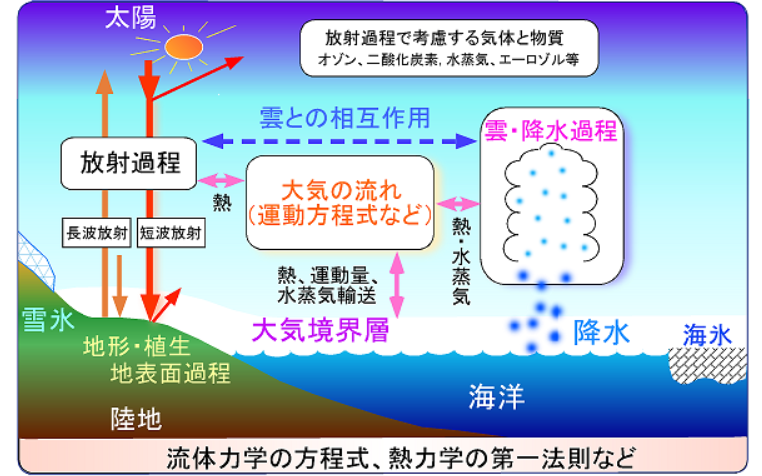
\includegraphics[width=0.8\textwidth]{./introduction/figs/numerical_weather_prediction.png.eps}
    \caption{数値予報の概要図\cite{KishochouNWP}}
    \label{fig:conventional-weather-forecast}
\end{figure}

\begin{figure}[bp]
    \centering
    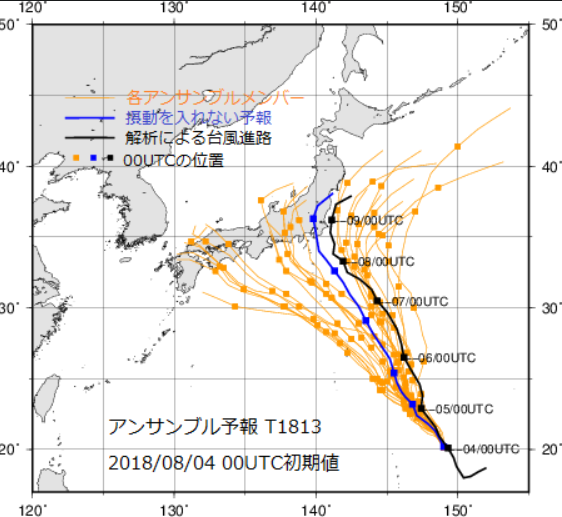
\includegraphics[width=0.7\textwidth]{./introduction/figs/ensemble.png.eps}
    \caption{アンサンブル予報から得られた台風進路の予報の例\cite{nwpensemble2018}}
    \label{fig:ensemble-forecast}
\end{figure}

\subsection{GraphCastによる気象予測 \label{subsec:graphcast}}
Google Deepmind社のLamら(2023)は,深層学習をベースにした全球中期予報モデルGraphCastを提案した\cite{Lam2023}.ここで中期予報とは,最大10日間までの予報を指している.彼らのモデルの概要図を図\ref{fig:graphcast_architecture}に示す.図\ref{fig:graphcast_architecture}(a),(b),(c)が示すようにGraphCastは,入力された時刻の気温,風速,海面温度,地面温度,降水量などの気象情報から1ステップ先の気象情報を予測しそれを繰り返すことで逐次将来の気象情報を予測をしていくモデルである.このモデルは図\ref{fig:graphcast_architecture}(d),(e),(f)が示すように,エンコーダ,プロセッサ,デコーダの3つの部分から成る.エンコーダは入力された気象情報をマルチメッシュグラフと呼ばれる構造に変換する.プロセッサではこのグラフ構造を用いて,図\ref{fig:graphcast_architecture}(g)に示すように遠近のいくつかの頂点から情報を伝達し各頂点の情報を更新する.デコーダはプロセッサの出力をグラフ構造から元の気象情報の形式に変換する.

\begin{figure}[bp]
    \centering
    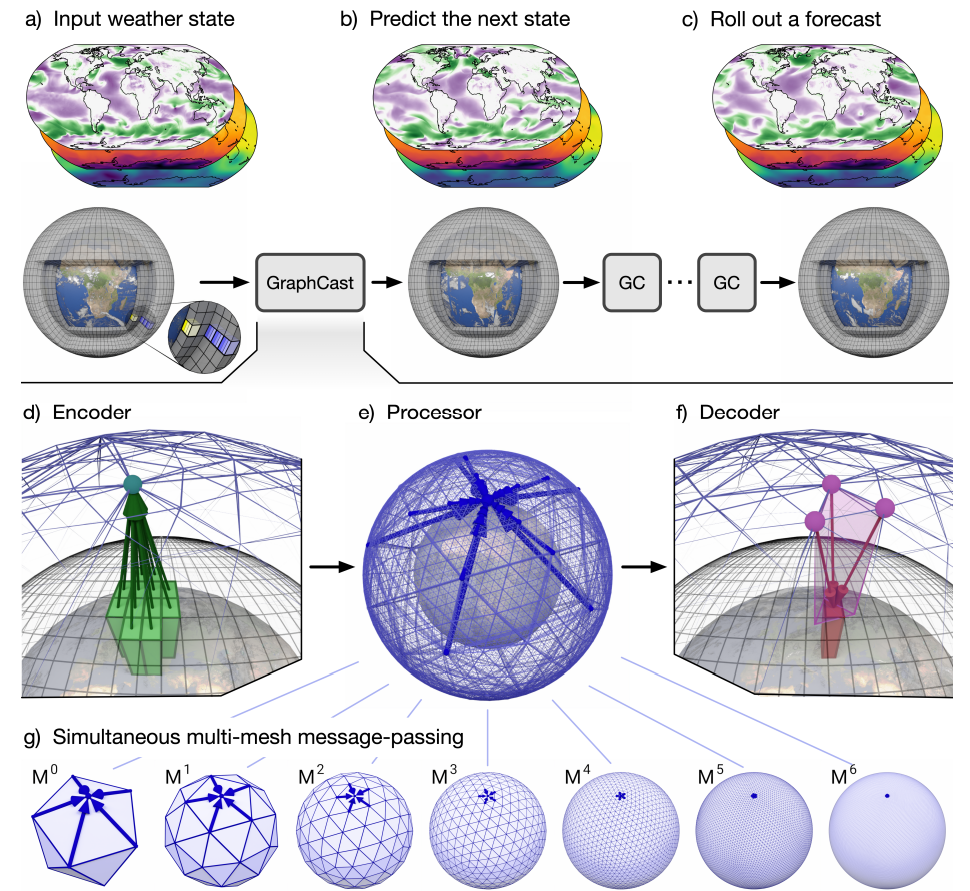
\includegraphics[width=0.9\textwidth]{./introduction/figs/graphcast-overview.png.eps}
    \caption{Lamら(2023)のモデルの概要図\cite{Lam2023} (a) 入力される気象情報 (b) 1ステップ先の予測された気象情報 (c) 数ステップ先の予測された気象情報 (d) エンコーダ (e) プロセッサ (f) デコーダ (g) マルチメッシュグラフが情報をやり取りする様子}
    \label{fig:graphcast_architecture}
\end{figure}

ECMWFで全球中期予報に用いられているHRESモデル\cite{HRES}に比べてGraphCastは$500\mathrm{hPa}$面のジオポテンシャル\cite{Geopotential}予測の二乗平均平方根誤差(Root Mean Squared Error, RMSE)が$7-14\%$低く,風速や気圧,温度などその他の多くの予測についても精度が上回った.また,図\ref{fig:cyclone_track}に示すように,特異的な気象現象であるサイクロンの軌跡予測についてもHRESモデルの精度を上回った.

彼らは,このモデルが10日分の予測をするのに単一のTPUプロセッサでも1分もかからないため,従来の手法に比べて計算量の観点においても大きいアドバンテージを有していると主張している.しかしモデルの学習には32個ものTPUプロセッサを1週間用いる必要があり,依然として計算規模が大きい.例えば日本近辺に限った局所的な予測をすることで計算量を減らそうとしても,局所的なマルチメッシュグラフを構成できないのでこの手法を適応することは難しいと推察される.

\begin{figure}[bp]
    \centering
    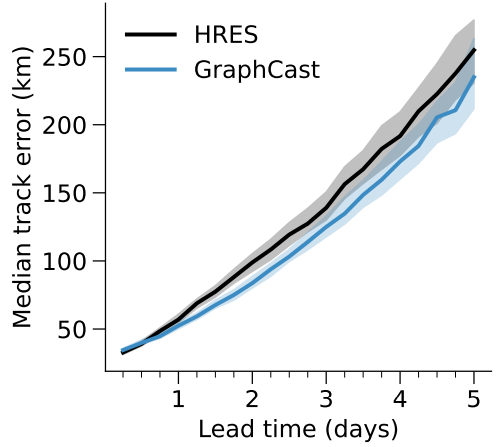
\includegraphics[width=0.4\textwidth]{./introduction/figs/cyclone_track.png.eps}
    \caption{GraphCastとHRESによるサイクロンの軌跡予測精度の比較\cite{CHEN2021114451}}
    \label{fig:cyclone_track}
\end{figure}

\subsection{CNNとLSTMを用いた正方形領域での風速予測 \label{subsec:chen2021}}
ここでは,深層学習の手法を用いて全球予測ではなく局所的な短期予測をするモデルを紹介する.Chenら(2021)は,CNN(Convolutional Neural Network)\cite{Yamashita2018}とLSTM(Long Short-Term Memory)\cite{10.1162/neco.1997.9.8.1735}を用いたモデルによる正方形領域での風速予測を行った\cite{CHEN2021114451}.彼らのモデル概要図を図\ref{fig:chen2021_architecture}に示す.この図において,エンコーダとデコーダの部分にCNNが用いられており,これにより正方形領域における格子点上の風速の空間的なパターンを学習している.また,エンコーダの出力をLSTMに入力し,更にその出力をデコーダに入力している.このLSTMのユニットにより,時間的なパターンも学習している.
\begin{figure}[bp]
    \centering
    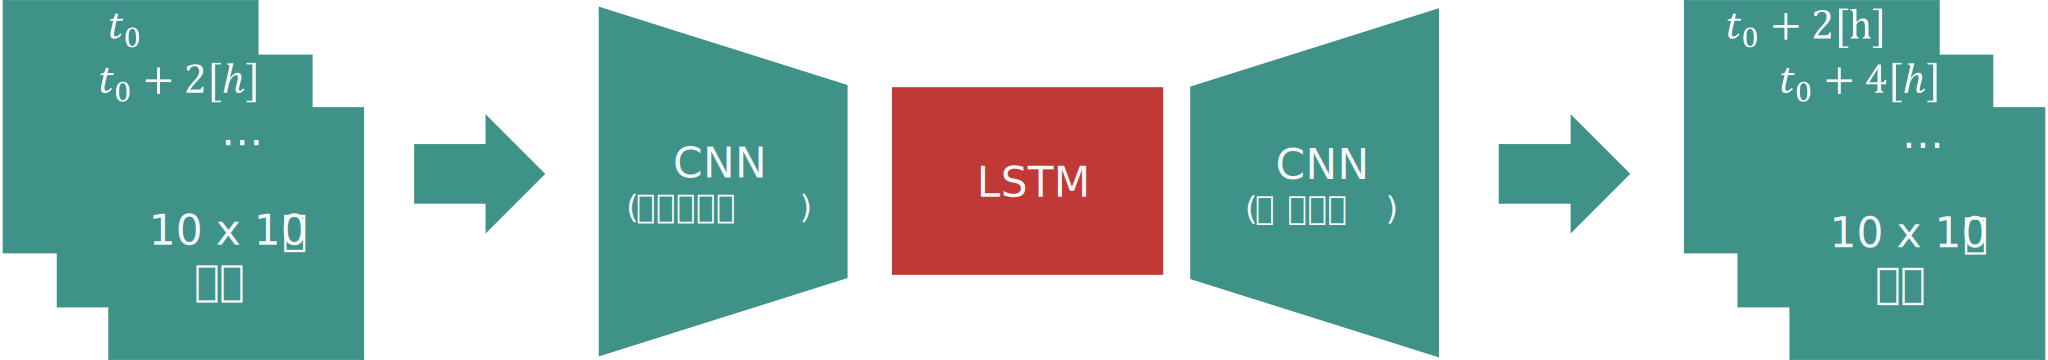
\includegraphics[width=0.9\textwidth]{./introduction/figs/chen2021_model_overview.svg.eps}
    \caption{Chenら(2021)のモデル概要図\cite{CHEN2021114451}}
    \label{fig:chen2021_architecture}
\end{figure}

このモデルを使って,彼らは図\ref{fig:chen2021_region}に示すようにアメリカのインディアナ州内部で,2km間隔の$10 \times 10$格子点上で2時間先の風速予測を行い,単にANN(Artificial Neural Network)\cite{485891}やLSTMのみを用いたモデルに比較して精度が向上することを示した.具体的には,全体の風速予測の平均絶対誤差(Mean Absolute Error, MAE)が$0.35 \mathrm{m/s}$減少し,これはPersistence モデル,ANNのみのモデル, LSTMのみのモデルの結果に比べてそれぞれ$32.7\%$, $28.8\%$, $18.9\%$低い値であると主張している.ここで,Persistence モデルとは,風速の時間変化を考慮せず,直前の風速をそのまま予測値とするモデルである.
\begin{figure}[bp]
    \centering
    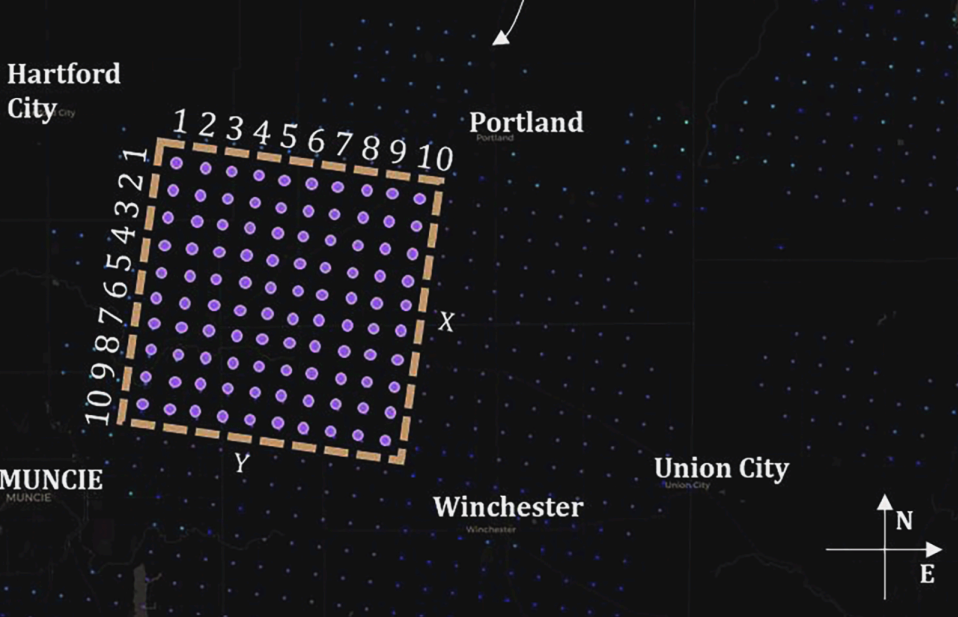
\includegraphics[width=0.8\textwidth]{./introduction/figs/chen2021_region.png.eps}
    \caption{Chenら(2021)が風速予測を行った範囲\cite{CHEN2021114451}}
    \label{fig:chen2021_region}
\end{figure}

\subsection{Physics-Informed Neural Networks \label{subsec:pinns}}
Raissi(2020)らは,物理学の知識をニューラルネットワークに組み込むことで,データが少ない場合でも高精度な予測を行うことができるPhysics-Informed Neural Networks(PINNs)というモデルを提案した\cite{PINNs2020}.このモデルは流体のシミュレーションに使われることが多く\cite{app13126892},ここでもその用途を想定する.彼らの提案したモデル概要図を図\ref{fig:pinns-overview}に示す.
\begin{figure}[bp]
    \centering
    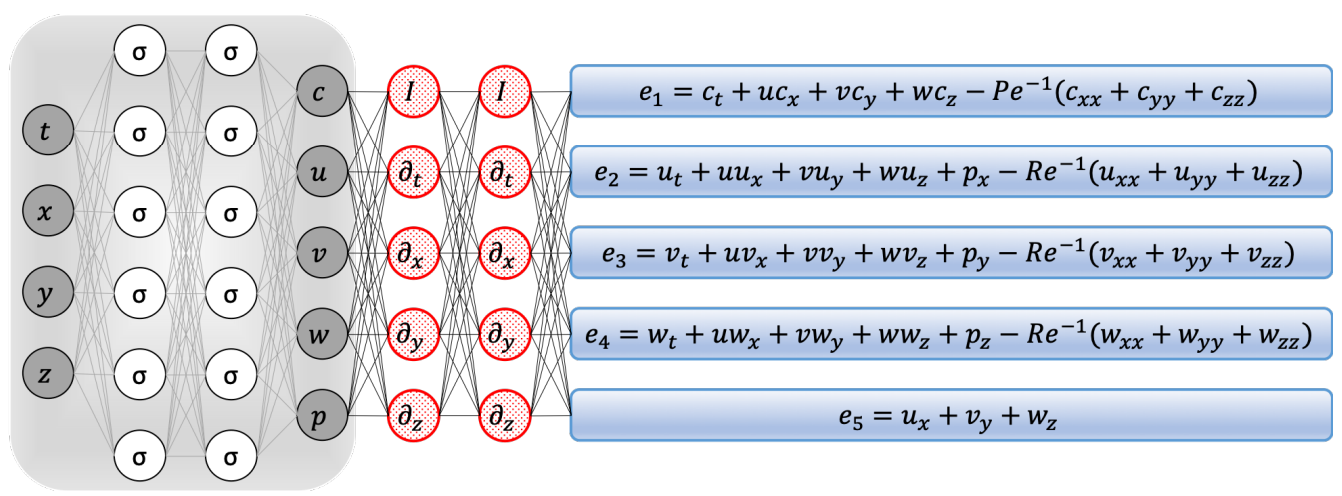
\includegraphics[width=0.9\textwidth]{./introduction/figs/PINNs_overview.png.eps}
    \caption{Raissiら(2020)のモデル概要図\cite{PINNs2020}}
    \label{fig:pinns-overview}
\end{figure}
この図が示すように,彼らのモデルは座標$x$,$y$,$z$と時刻$t$を入力とし,それに対応する流体のパッシブスカラーの濃度$c$,流体の速度$u$,$v$,$w$,そして流体の圧力$p$を出力する.なおパッシブスカラーとは,流体の流れによって変化するが流体の流れに影響を与えない物理量のことであり,例えば流体に溶けた微量な染料の濃度などが挙げられる\cite{Lesieur1990}.

彼らのモデルは,損失関数(\ref{subsection:neuron-principles}項参照)に物理的な微分方程式からどれだけモデルの出力が乖離しているかを表す項を組み込むことで,物理法則を満たすように学習をする.図\ref{fig:pinns-overview}中では$e_1$,$e_2$,$e_3$,$e_4$,$e_5$がこの項に当たる.このとき,物理量の座標微分や時間微分は,\ref{subsection:automatic-differentiation}項に述べるように自動微分を使って導くことができる.実測データが少ない場合でも,それ以外の座標と時刻を入力した場合の損失が小さくなるようにすれば,モデルの出力は物理法則に従うと彼らは主張している.

%この手法では,物理的な外力や拘束条件が既知の場合では有効であるが,例えば大気のように外力や拘束条件が不明または特定が困難な場合には損失関数をどう定めればよいのかわからず,適用するのが難しいという問題点がある. %これは良くない気がする.なぜなら,そもそもデータセットが少ない場合に適応するのが目的だから,データセットが多い場合はそもそもPINNsを使う必要がないから




\section{研究目的}
本研究では\ref{subsec:conventional-weather-forecast}項や\ref{subsec:graphcast}項で述べたような全球予測を行うモデルではなく,\ref{subsec:chen2021}項で述べたChenら(2021)の研究と同様に,日本を含む長方形領域における格子点上での短期風速予測を行うモデルを扱う.そして,ニューラルネットワークの構造にLBMを組み込むことで,それらが持つ並列計算との相性の良さを活かしつつ,流体力学の知見を用いて風速予測の精度を向上させることを目的とする.
また\ref{subsec:pinns}項で述べたRaissiら(2020)の研究とは対照的に,大気の風速予測のようにデータセットが十分あるが外力や拘束条件が不明または特定が困難な場合にも,物理法則を利用できるモデルを提案することも目的としている.

\section{論文構成}
本論文では,第\ref{section:deep-learning}節で深層学習の,第\ref{section:lbm}節で格子ボルツマン法の数理的な原理を解説し,それらを踏まえて第\ref{chap:how-to-assemble}章で提案モデルでは格子ボルツマン法をどのように深層学習モデルに組み込んだのかを解説する.第\ref{chap:experiments}章では,提案モデルの有効性を検証するため,日本近辺の風速予測を行い,従来研究のモデルと比較検討をする.

\chapter{原理 \label{chap:principles}}
\section{深層学習 \label{section:deep-learning}}
深層学習は機械学習の一分野であり,複数の隠れ層から成るニューラルネットワークを使用して高度なパターン認識や特徴抽出を行う手法である.この章では最も単純で典型的な深層学習のアーキテクチャを説明する.
\if0
どのくらい書くべきか?どう書くべきか?
この原理の章はそもそも自分のモデルを説明するときに使うものであって,先に自分のモデルについて書いたほうがやりやすいかもしれん.
- 読者にどの程度の前提知識を求めるべきか.
\fi

図\ref{fig:dnn-architecture}に示す通り,深層学習は入力層,隠れ層,出力層から成るニューラルネットワークで表される.入力層は入力データを受け取り,隠れ層は入力層から出力を受け取り,出力層は隠れ層の出力を受け取る.隠れ層は複数存在し,それぞれの隠れ層は前の隠れ層の出力を受け取る.ここで,各層は複数のニューロンからなり,各ニューロンは入力された実数値に活性化関数を適用した値を出力する.図\ref{fig:dnn-architecture}中の破線矢印が活性化関数に対応する.そしてその入力値は,前の層のニューロンの出力に重みをかけたものの和にバイアスを加えた値である.これは図\ref{fig:dnn-architecture}中の実線矢印に対応する.十分な隠れ層を持ち,重みが適切に調節されたニューラルネットワークは任意の関数を近似することができることが知られている\cite{Hornik1989MultilayerFN}.

\begin{figure}[btp]
  \centering
  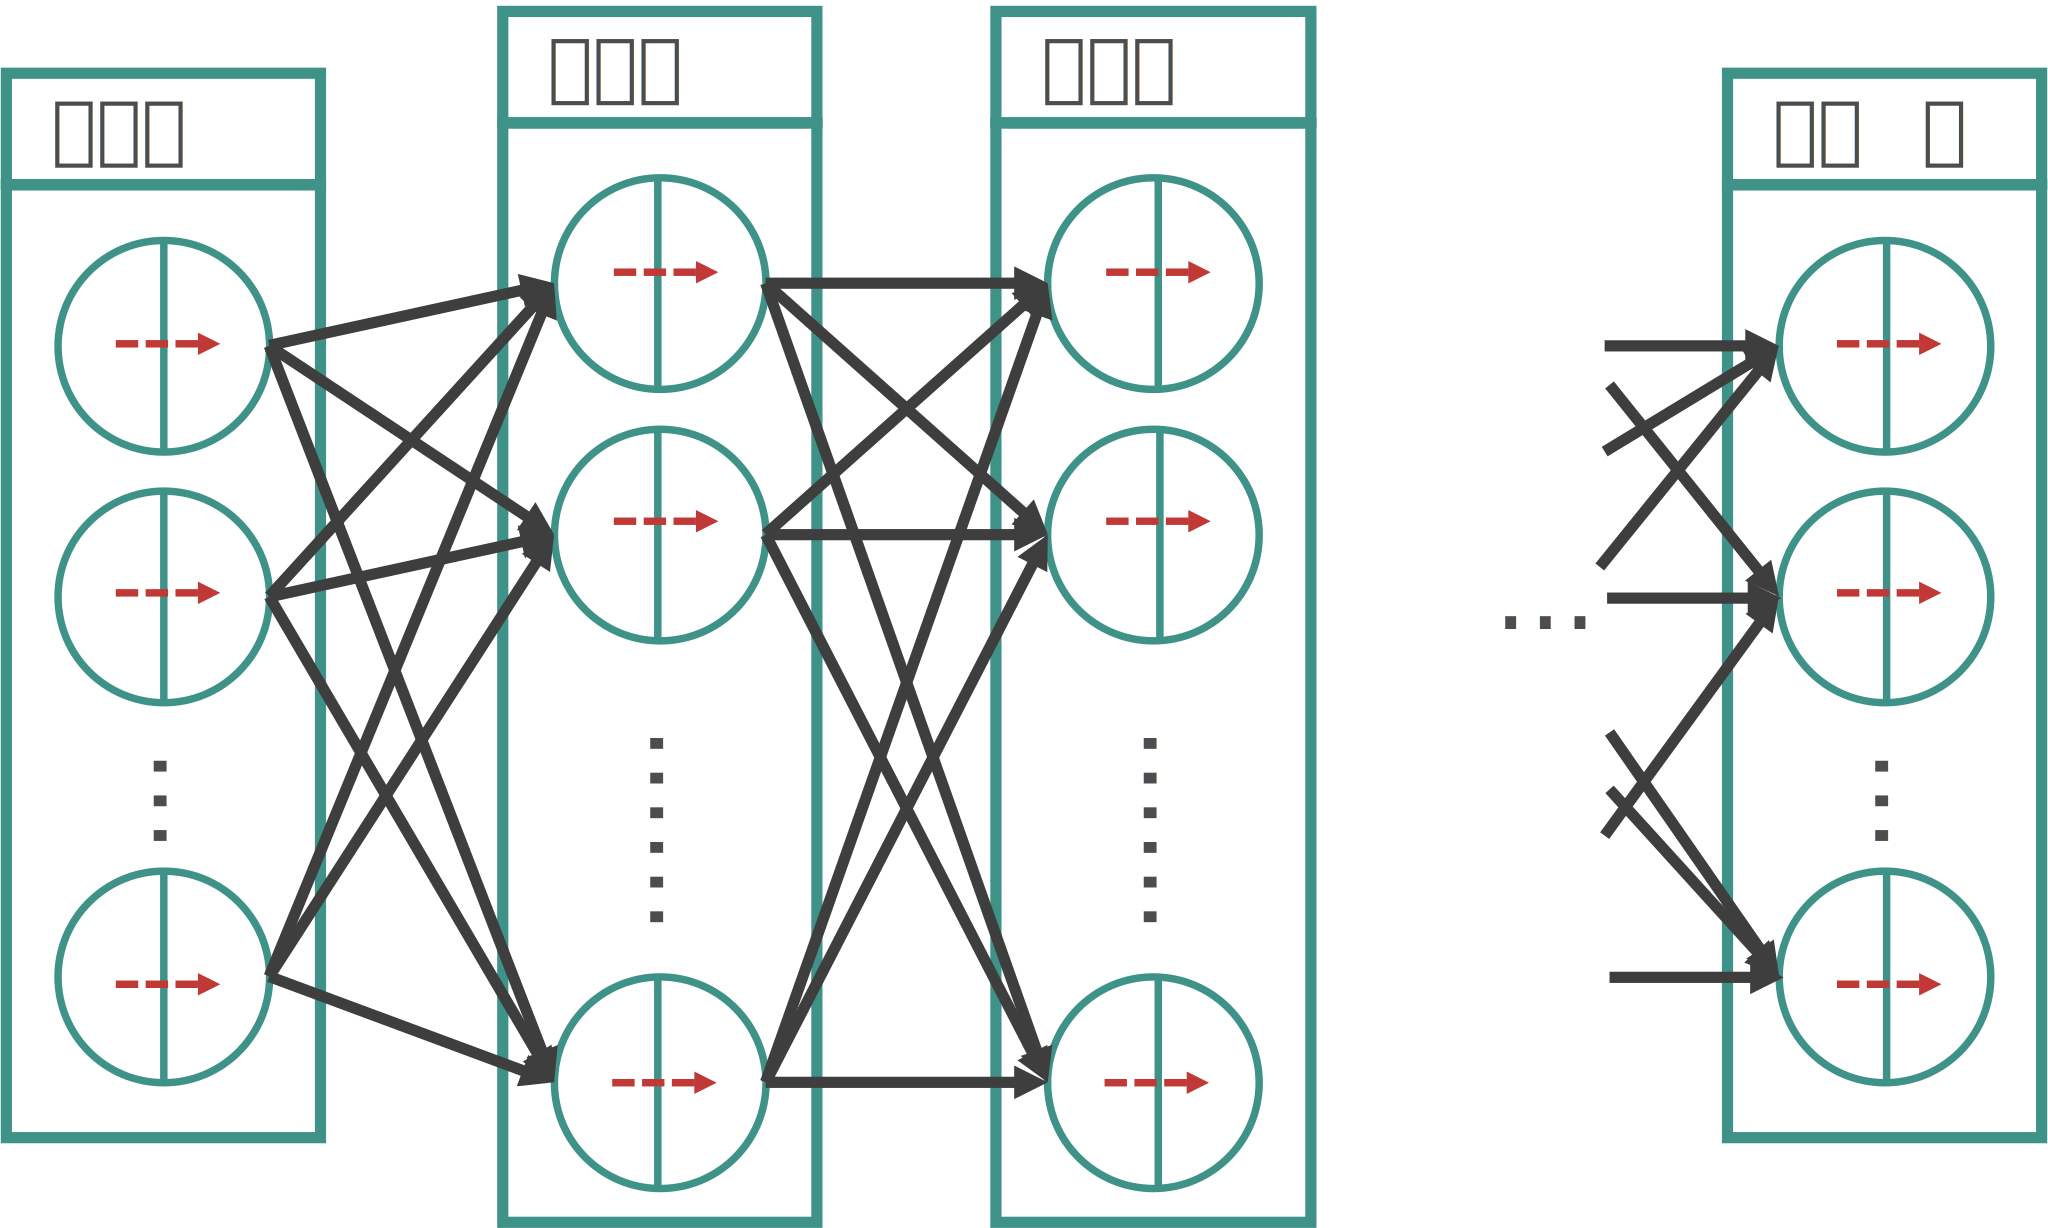
\includegraphics[width=0.7\linewidth]{./principles/figs/dnn_overview.svg.eps}
  \caption{深層学習のアーキテクチャ}
  \label{fig:dnn-architecture}
\end{figure}

\subsection{ニューラルネットワークの計算原理 \label{subsection:neuron-principles}}
より詳しく原理を説明する.合計で$m$層になるニューラルネットワークを考える.まず,入力層のニューロンの数を$n^{(1)}$とし,第$j$ ($1 \leq j \leq n^{(1)}$)ニューロンへの入力を$y_j^{(1)} \in \mathbb{R}$,ニューロンからの出力を$z_j^{(1)} \in \mathbb{R}$とする.$y_j^{(1)}$は入力データの第$j$成分を意味する.また,$z_j^{(1)}$は$y_j^{(1)}$に活性化関数$f^{(1)}: \mathbb{R} \rightarrow \mathbb{R}$を適用した値である.つまり,
\begin{equation}
  z_j^{(1)} = f^{(1)}(y_j^{(1)})
  \label{eq:deep-learning-input-layer}
\end{equation}
である.
次に,中間層または出力層である第$k$ $(2 \leq k \leq m)$層のニューロンの数を$n^{(k)}$とし,第$j$ $(1 \leq j \leq n^{(k)})$ニューロンへの入力を$y_j^{(k)} \in \mathbb{R}$,ニューロンからの出力を$z_j^{(k)} \in \mathbb{R}$とすると,これらは以下のように表される.
\begin{equation}
  y_j^{(k)} = \sum_{i=0}^{n^{(k-1)}} w_{ij}^{(k)} z_i^{(k-1)}
  \label{eq:deep-learning-neuron-input}
\end{equation}
\begin{equation}
  z_j^{(k)} = f^{(k)}(y_j^{(k)})
  \label{eq:deep-learning-neuron-output}
\end{equation}
ここで,$w_{ij}^{(k)} \in \mathbb{R}$は第$k-1$層の第$i$ニューロンから第$k$層の第$j$ニューロンへの重み,$f^{(k)}: \mathbb{R} \rightarrow \mathbb{R}$は活性化関数である.ただし,$f^{(m)}$は恒等関数とする.活性化関数は通常非線形関数であり,シグモイド関数やReLU関数などが用いられる.またここでは$z_0^{(k-1)} = 1$とすることで,バイアス$w_{0j}^{(k)}$を導入する.

以上から,ニューラルネットワークに$y_1^{(1)}, \dots, y_{n^{(1)}}^{(1)}$を入力すると式(\ref{eq:deep-learning-input-layer}), (\ref{eq:deep-learning-neuron-input}), (\ref{eq:deep-learning-neuron-output})
によって順次計算が行われ,$z_1^{(m)}, \dots, z_{n^{(m)}}^{(m)}$が出力されることがわかる.続いて,これをどのように目的の出力に近づけるかを考える.

目的の出力を$\hat{z}_0^{(m)}, \dots, \hat{z}_{n^{(m)}}^{(m)}$とする.このとき,出力層のニューロンの出力と目的の出力の誤差を表す二乗損失関数は次のように表される(これは単に損失とも呼ばれる).
\begin{equation}
  E = \frac{1}{2} \sum_{j=1}^{n^{(m)}} \left( z_j^{(m)} - \hat{z}_j^{(m)} \right)^2
  \label{eq:deep-learning-loss}
\end{equation}

これを最小化するように各層の重みを調節することで,ニューラルネットワークは目的の出力に近づく.ここでは最も単純な勾配降下法を用いる.まず,隠れ層及び出力層に接続する重み$w_{ij}^{(k)}$ $(2 \leq k \leq m)$の誤差$E$に対する勾配は$\partial E / \partial w_{ij}^{(k)}$で表され,これにより重みを次のように更新すると誤差が減少することが分かる.
\begin{equation}
  w_{ij}^{(k)} \leftarrow w_{ij}^{(k)} - \eta \frac{\partial E}{\partial w_{ij}^{(k)}}
  \label{eq:deep-learning-gradient-descent}
\end{equation}
ここで,$\eta$は学習率と呼ばれる$0$以上の実数である.以下では$\partial E / \partial w_{ij}^{(k)}$を求めることを考える.そのために準備としてひとつ記号を定義する.$\delta_j^{(k)}$を第$k$層の第$j$ニューロンの誤差といい,以下で定義する.
\begin{equation}
  \delta_j^{(k)} = \frac{\partial E}{\partial u_j^{(k)}}
  \label{eq:deep-learning-delta}
\end{equation}
これを用いて$\partial E / \partial w_{ij}^{(k)}$を表し,最後に誤差を求める.

$2 \leq k \leq m$とする.式(\ref{eq:deep-learning-neuron-output}), (\ref{eq:deep-learning-delta})より,$\partial E / \partial w_{ij}^{(k)}$は次のように表される.
\begin{equation}
  \frac{\partial E}{\partial w_{ij}^{(k)}} =
  \frac{\partial E}{\partial u_j^{(k)}} \frac{\partial u_j^{(k)}} {\partial w_{ij}^{(k)}} =
  \delta_j^{(k)} \frac{\partial u_j^{(k)}} {\partial w_{ij}^{(k)}}
  \label{eq:deep-learning-middle-layer}
\end{equation}
そして,式(\ref{eq:deep-learning-neuron-input})より,$\partial u_j^{(k)} / \partial w_{ij}^{(k)}$は次のように表される.
\begin{equation}
  \frac{\partial u_j^{(k)}} {\partial w_{ij}^{(k)}} =
  \frac{ \partial \left( \sum_{i=0}^{n^{(k-1)}} w_{ij}^{(k)} z_i^{(k-1)} \right)} {\partial w_{ij}^{(k)}} =
  z_i^{(k-1)}
  \label{eq:deep-learning-middle-layer-2}
\end{equation}
したがって,式(\ref{eq:deep-learning-middle-layer}), (\ref{eq:deep-learning-middle-layer-2})より,
\begin{equation}
  \frac{\partial E}{\partial w_{ij}^{(k)}} =
  \delta_j^{(k)} z_i^{(k-1)}
  \label{eq:deep-learning-middle-layer-3}
\end{equation}
となる.

最後に誤差を求める.まず,出力層の誤差$\delta_j^{(m)}$は式(\ref{eq:deep-learning-delta}), (\ref{eq:deep-learning-loss})より次のように表される.
\begin{equation}
  \delta_j^{(m)} = \frac{\partial E}{\partial u_j^{(m)}} =
  \frac{\partial E}{\partial z_j^{(m)}} =
  \frac{\partial \left( \frac{1}{2} \sum_{j=1}^{n^{(m)}} \left( z_j^{(m)} - \hat{z}_j^{(m)} \right)^2 \right)} {\partial z_j^{(m)}} =
  z_j^{(m)} - \hat{z}_j^{(m)}
  \label{eq:deep-learning-output-error}
\end{equation}
続いて,$2 \leq k \leq m-1$に対して,第$k$層の誤差$\delta_j^{(k)}$は次のように表される.
\begin{equation}
  \begin{split}
  \delta_j^{(k)} &= \frac{\partial E}{\partial u_j^{(k)}} =
  \sum_{i=1}^{n^{(k+1)}} \frac{\partial E}{\partial u_i^{(k+1)}} \frac{\partial u_i^{(k+1)}} {\partial u_j^{(k)}} \\ &=
  \sum_{i=1}^{n^{(k+1)}} \delta_i^{(k+1)} \frac{\partial u_i^{(k+1)}} {\partial z_j^{(k)}} \frac{\partial z_j^{(k)}} {\partial u_j^{(k)}} \\ &=
  \sum_{i=1}^{n^{(k+1)}} \delta_i^{(k+1)} w_{ji}^{(k+1)} f^{(k)\prime}(y_j^{(k)})
  \end{split}
  \label{eq:deep-learning-middle-error}
\end{equation}

以上より,式(\ref{eq:deep-learning-output-error}), (\ref{eq:deep-learning-middle-error})を用いて$\delta_j^{(k)}$を順次計算し,さらに式(\ref{eq:deep-learning-middle-layer-3})を用いて$\partial E / \partial w_{ij}^{(k)}$を順次計算することで,式(\ref{eq:deep-learning-gradient-descent})によって重みを更新することができる.

\subsection{自動微分 \label{subsection:automatic-differentiation}}
\ref{subsection:neuron-principles}項では,ニューラルネットワークの重みを更新するために,誤差を逐次的に求めていく必要があることを述べた.しかし,ニューラルネットワークのモデルが複雑化するに従って,この数式を手作業で計算することは困難になってくる.そこで,自動微分と呼ばれる手法を用いる.
一般的にコンピュータ上で表される関数は,基本的には四則演算や三角関数,指数関数などの初等関数の合成で表される\cite{10.5555/3122009.3242010}.自動微分では,このような基本的な関数の微分をあらかじめ定義しておき,合成関数の微分を関数の微分の積で表すことで計算する\cite{10.5555/3122009.3242010}.PyTorch\cite{NEURIPS2019-9015}やTensorFlow\cite{tensorflow2015-whitepaper}などの深層学習フレームワークでは,この自動微分が実装されているため,複雑なモデルでも容易に実装することができる.

\section{格子ボルツマン法 \label{section:lbm}}

格子ボルツマン法(LBM, Lattice Boltzmann Method)は数値流体力学の一手法である.流体を有限種類の速度を持つ仮想粒子の集合とみなし,その分布関数を時空間で離散化したものに対して並進と衝突と呼ばれる操作を逐次施すことで流体の動きを表現する.この章では,LBMの基本的な原理を説明する.

等温場の格子流体モデルとして,ここではD2Q9モデルを考える.D2Q9モデルは,仮想粒子の速度ベクトルが以下の式に示す9種類である二次元空間格子モデルである.
\begin{equation}
  \bm{v} = \left( \pm 1, \pm 1 \right), \left( \pm 1, 0 \right), \left( 0, \pm 1 \right), \left( 0, 0 \right)
  \label{eq:lbm-velocity}
\end{equation}
ただし,複号任意である.これは図\ref{fig:d2q9}に示すとおり,速度ベクトルは格子の中心からのオフセットで表されることを意味している.この下で,分布関数$f(\bm{x}, \bm{v}, t)$は無次元座標$\bm{x} \in \mathbb{R}^2$,無次元時刻$t \in \mathbb{R}$における速度$\bm{v}$の粒子数を表す.すると,これは任意の$\bm{v}$について以下の離散ボルツマン方程式に従う\cite{Inamuro1990NumericalSO}.
\begin{equation}
  \mathrm{Sh} \frac{\partial f(\bm{x}, \bm{v}, t)}{\partial t} + \bm{v} \cdot \nabla f(\bm{x}, \bm{v}, t) = \frac{1}{\epsilon} \Omega_{\bm{v}}\left[ f(\bm{x}, \bm{v}', t) \right]
  \label{eq:lbm-discrete-boltzmann}
\end{equation}
\begin{figure}[btp]
  \centering
  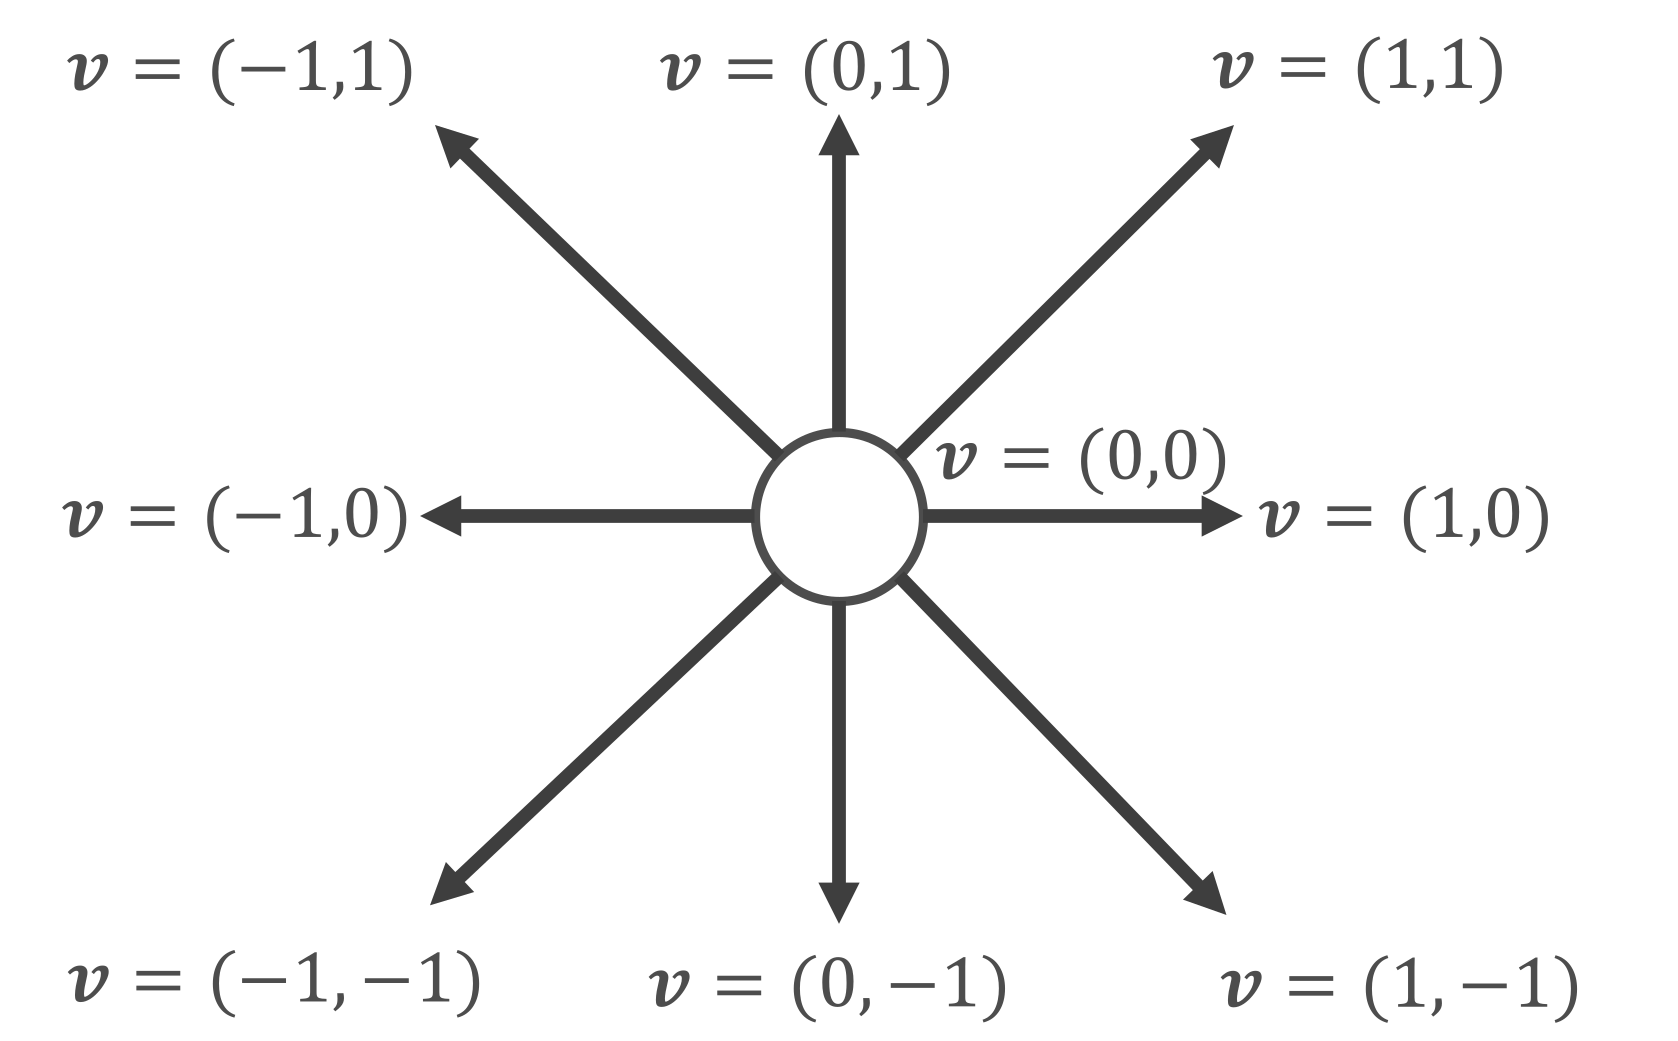
\includegraphics[width=0.6\linewidth]{./principles/figs/lbm_d2q9.svg.eps}
  \caption{D2Q9モデルの速度ベクトル}
  \label{fig:d2q9}
\end{figure}
ここで,$\mathrm{Sh}$はストローハル数,$\epsilon$はクヌーセン数,$\Omega_{\bm{v}}$は仮想粒子の衝突による増減を表す衝突演算子である.ただし,$\bm{v}'$はパラメータ化されておりすべての$\bm{v}'$について演算を行うと約束する.続いて,空間と時間を$\Delta x = 1/\epsilon$, $\Delta t = \mathrm{Sh} \Delta x$によってそれぞれ分割し,式(\ref{eq:lbm-discrete-boltzmann})を時空間について一次前進差分によって近似すると次式を得る.
\begin{equation}
  f(\bm{x}+\bm{v}\Delta t, \bm{v}, t+\Delta t) - f(\bm{x}, \bm{v}, t) = \Omega_{\bm{v}}\left[ f(\bm{x}, \bm{v}', t) \right]
  \label{eq:lbm-lattice-boltzmann}
\end{equation}
また,離散化された時空間上での分布関数から,流体の巨視的な密度$\rho(\bm{x}, t)$と巨視的な流速$\bm{u}(\bm{x}, t)$は以下のように定義される.
\begin{equation}
  \rho(\bm{x}, t) = \sum_{\bm{v}} f(\bm{x}, \bm{v}, t)
  \label{eq:lbm-macro-density}
\end{equation}
\begin{equation}
  \rho(\bm{x}, t) \bm{u}(\bm{x}, t) = \sum_{\bm{v}} \bm{v} f(\bm{x}, \bm{v}, t)
  \label{eq:lbm-macro-velocity}
\end{equation}
式(\ref{eq:lbm-lattice-boltzmann})において,左辺が並進,右辺が衝突を表していることに注意されたい.この右辺に次式で表されるBGK(Bhatnagar-Gross-Krook)モデルと呼ばれる衝突演算子\cite{PhysRev.94.511}を導入する.
\begin{equation}
  \Omega_{\bm{v}}\left[ f(\bm{x}, \bm{v}', t) \right] = -\frac{1}{\tau} \left[ f(\bm{x}, \bm{v}, t) - f^{eq}(\bm{x}, \bm{v}, t) \right]
  \label{eq:lbm-bgk}
\end{equation}
ここで,$\tau$は流体の無次元緩和時間,$f^{eq}(\bm{x}, \bm{v}, t)$は局所平衡分布関数と呼ばれる関数である.式(\ref{eq:lbm-bgk})を式(\ref{eq:lbm-lattice-boltzmann})に代入すると,次式を得る.
\begin{equation}
  f(\bm{x}+\bm{v}\Delta t, \bm{v}, t+\Delta t) = f(\bm{x}, \bm{v}, t) - \frac{1}{\tau} \left[ f(\bm{x}, \bm{v}, t) - f^{eq}(\bm{x}, \bm{v}, t) \right]
  \label{eq:lbm-bgk-lattice-boltzmann}
\end{equation}
最後に,局所平衡分布関数を求める.この関数は
\begin{equation}
  \rho(\bm{x}, t) = \sum_{\bm{v}} f^{eq}(\bm{x}, \bm{v}, t)
  \label{eq:lbm-eq-macro-density}
\end{equation}
\begin{equation}
  \rho(\bm{x}, t) \bm{u}(\bm{x}, t) = \sum_{\bm{v}} \bm{v} f^{eq}(\bm{x}, \bm{v}, t)
  \label{eq:lbm-eq-macro-velocity}
\end{equation}
を満たす必要がある.これらを満たす局所平衡分布関数はマクスウェル分布\cite{Asakura1989}において$|\bm{u}|$が二次の項まで展開すると得られて,以下のように定義される.
\begin{equation}
  f^{eq}(\bm{x}, \bm{v}, t) = c(\bm{v}) \rho(\bm{x}, t) \left[ 1 + 3\bm{v} \cdot \bm{u}(\bm{x}, t) + \frac{9}{2}(\bm{v} \cdot \bm{u}(\bm{x}, t))^2 - \frac{3}{2}\bm{u}(\bm{x}, t)^2 \right]
  \label{eq:lbm-eq-1}
\end{equation}
ただし,式(\ref{eq:lbm-eq-macro-density}), (\ref{eq:lbm-eq-macro-velocity}), (\ref{eq:lbm-eq-1})内の$\rho(\bm{x}, t)$, $\bm{u}(\bm{x}, t)$はそれぞれ式(\ref{eq:lbm-macro-density}), (\ref{eq:lbm-macro-velocity})で求めた値を用いる.また,$c(\bm{v})$は速度ベクトル$\bm{v}$に対する重みであり,D2Q9モデルでは
\begin{equation}
  c(\bm{v}) = \left\{
    \begin{array}{ll}
      4/9 & (\bm{v} = (0, 0)) \\
      1/9 & (\bm{v} = (\pm 1, 0), (0, \pm 1)) \\
      1/36 & (\bm{v} = (\pm 1, \pm 1))
    \end{array}
  \right.
  \label{eq:lbm-weight}
\end{equation}
と求められる.以上の式(\ref{eq:lbm-bgk-lattice-boltzmann}), (\ref{eq:lbm-eq-1}), (\ref{eq:lbm-macro-density}), 及び(\ref{eq:lbm-macro-velocity})によりLBMの基本的な計算スキームが構成された.これらの計算スキームはChapman-Enskog展開によってナビエ・ストークス方程式を空間二次精度で再現することが知られている\cite{Inamuro2020}.

本研究においては時空間間隔をリスケールし,$\Delta x = 1$, $\Delta t = 1$として計算を行った.その上で式(\ref{eq:lbm-bgk-lattice-boltzmann})は次のように並進と衝突の式に分離することができる.
\begin{equation}
  f'(\bm{x}+\bm{v}, \bm{v}, t)
  = f(\bm{x}, \bm{v}, t)
  \label{eq:lbm-streaming}
\end{equation}
\begin{equation}
  f(\bm{x}, \bm{v}, t+1)
  = f'(\bm{x}, \bm{v}, t) - \frac{1}{\tau} \left[ f'(\bm{x}, \bm{v}, t) - f^{eq}(\bm{x}, \bm{v}, t) \right]
  \label{eq:lbm-collision}
\end{equation}
このとき,式(\ref{eq:lbm-eq-1})は次のように表される.
\begin{equation}
  f^{eq}(\bm{x}, \bm{v}, t) = c_i(\bm{v}) \rho'(\bm{x}, t) \left[ 1 + 3\bm{v} \cdot \bm{u}'(\bm{x}, t) + \frac{9}{2}(\bm{v} \cdot \bm{u}'(\bm{x}, t))^2 - \frac{3}{2}\bm{u}'(\bm{x}, t)^2 \right]
  \label{eq:lbm-eq}
\end{equation}



\chapter{格子ボルツマン法を組み込んだ深層学習モデル\label{chap:how-to-assemble}}
この章では,提案モデルの概要とより具体的な原理について説明する.

\section{提案モデルの概要}
提案モデルの概要図を図\ref{fig:overview}に示す.この図が示すように,提案モデルはLBMをベースとしている.その並進と衝突の計算に重みを導入し,予測速度と圧力に対する実測速度と圧力との誤差からその重みを誤差逆伝播法によって学習することで,座標に依存する流体の振る舞いを精度良くシミュレーションすることを試みる.学習の流れを詳述する.まずある無次元時刻$t_0$の各格子点上での流体の速度,圧力から,仮想粒子の分布$f(\bm{x}, \bm{v}, t_0)$を導出する.そこから$\Delta T$ステップに亘り,並進と衝突の計算によって仮想粒子の分布$f'(\bm{x}, \bm{v}, t_0+i)$, $f(\bm{x}, \bm{v}, t_0+i+1) \hspace{10pt}(i=0,...,\Delta T - 1)$を逐次的に得る.最終的な時刻$t_1 = t_0 + \Delta T$での分布$f(\bm{x}, \bm{v}, t_1)$から巨視的な流体の速度と圧力を算出し,これと実測流体の速度と圧力との誤差から,各ステップに導入した重みを誤差逆伝播法によって学習する.
\begin{figure}[tbp]
  \centering
  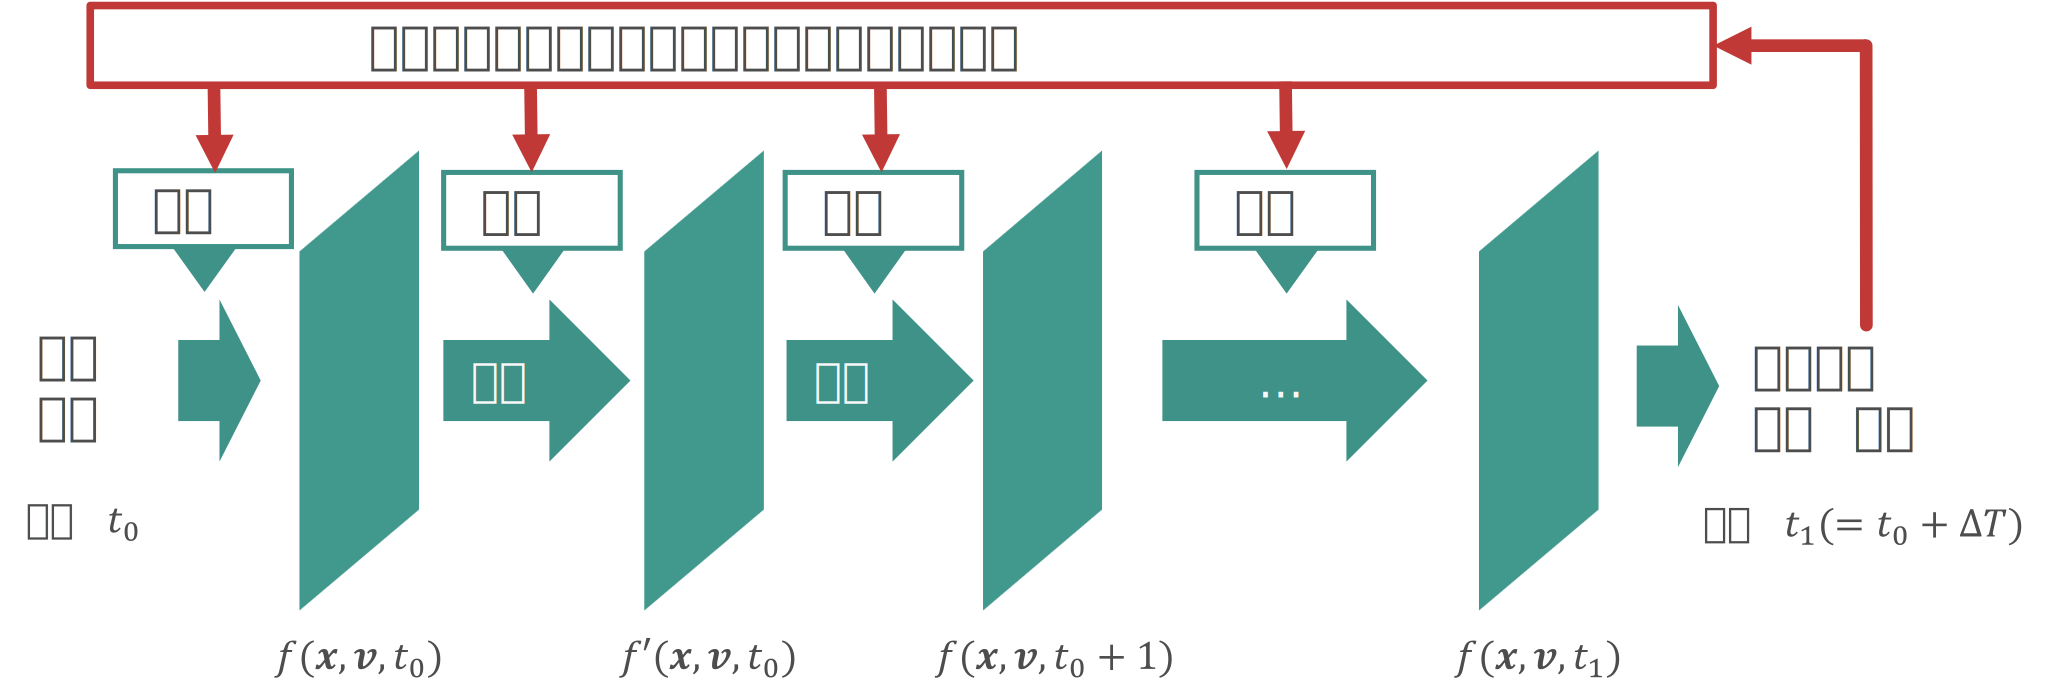
\includegraphics[width=13cm]{./how_to_assemble/figs/model_overview.svg.eps}
  \caption{提案モデルの概要図}
  \label{fig:overview}
\end{figure}

\section{提案モデルの原理}
この節では,具体的にどのようにLBMに重みを導入し学習を行うか,その原理について説明する.まずは図\ref{fig:model-comparison}(a)で表されるように,ある一時刻のデータのみが入力されたときにその$\Delta T$後の流速のみを予想する時系列性のないモデルを説明する.その後,図\ref{fig:model-comparison}(b)で表されるように$\Delta T$おきの時系列データが入力されたとき,それぞれの時刻に対して$\Delta T$後の時系列データを予測するモデルを説明する.

\begin{figure}[tbp]
  \centering
  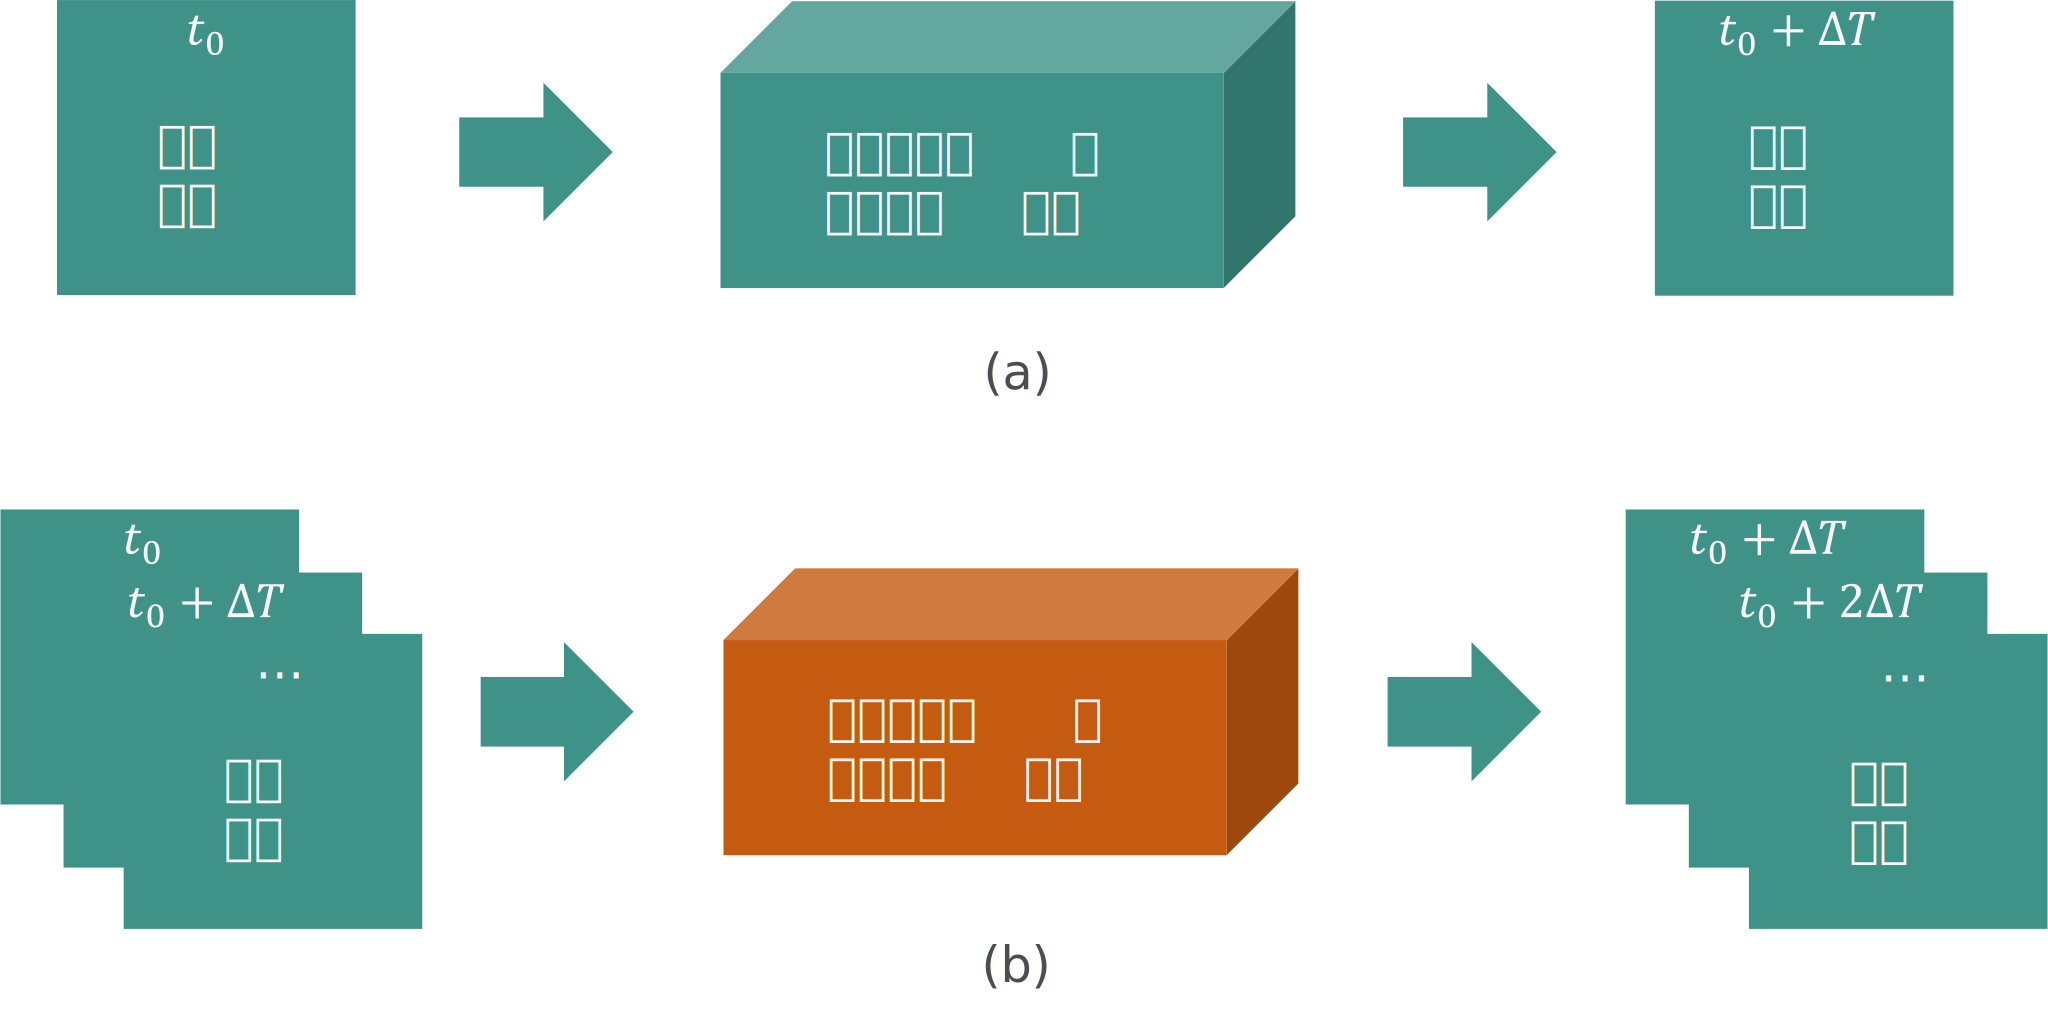
\includegraphics[width=13cm]{./how_to_assemble/figs/time_series_comparison.svg.eps}
  \caption{時系列性のないモデルと時系列性のあるモデルの比較 (a)時系列性のないモデルの入出力 (b)時系列性のあるモデルの入出力}
  \label{fig:model-comparison}
\end{figure}

\subsection{時系列性のないモデル\label{subsection:time-series-less-model}}
時系列性のないモデルでは,ある無次元時刻$t_0$での流速$\hat{\bm{u}}(\bm{x}, t_0)$と圧力$\hat{\rho}(\bm{x}, t_0)$のデータが入力されたときに時刻$t_1 = t_0 + \Delta T$での流速$\hat{\bm{u}}(\bm{x}, t_1)$と圧力$\hat{\rho}(\bm{x}, t_1)$を予測する.まずLBMの並進と衝突の式にどのように重みを導入するかを説明する.

LBMの並進は,仮想粒子の分布関数$f(\bm{x}, \bm{v}, t)$を用いて以下のように表された(再掲).
\begin{equation}
  f'(\bm{x}+\bm{v}, \bm{v}, t)
  = f(\bm{x}, \bm{v}, t)
  \tag{\ref{eq:lbm-streaming}}
\end{equation}

この式に重み$w'_{\rm{const}}(\bm{x}, \bm{v}, t)$, $w'_{\rm{fprev}}(\bm{x}, \bm{v}, t)$を導入する.重みを導入することで,仮想粒子の分布関数$f(\bm{x}, \bm{v}, t)$を並進させる際に,仮想粒子の流入や流出を表現することができる.重みを導入した並進の式は以下のように表される.
\begin{equation}
  f'(\bm{x}+\bm{v}, \bm{v}, t) = 
  w'_{\rm{const}}(\bm{x}, \bm{v}, t) + 
  w'_{\rm{fprev}}(\bm{x}, \bm{v}, t) f(\bm{x}, \bm{v}, t)
  \label{eq:weighted-streaming}
\end{equation}

また,衝突の式は以下のように表された(再掲).
\begin{equation}
  f(\bm{x}, \bm{v}, t+1) = 
  f'(\bm{x}, \bm{v}, t) - 
  \frac{1}{\tau} \left[ 
    f'(\bm{x}, \bm{v}, t) - f^{eq}(\bm{x}, \bm{v}, t) 
  \right]
  \tag{\ref{eq:lbm-collision}}
\end{equation}

\begin{equation}
  f^{eq}(\bm{x}, \bm{v}, t) = 
  c_i(\bm{v}) \rho'(\bm{x}, t) \left[ 
    1 
    + 3\bm{v} \cdot \bm{u}'(\bm{x}, t) 
    + \frac{9}{2}(\bm{v} \cdot \bm{u}'(\bm{x}, t))^2 
    - \frac{3}{2}\bm{u}'(\bm{x}, t)^2 
  \right]
  \tag{\ref{eq:lbm-eq}}
\end{equation}

これらの式にも重み$w_{\rm{fprev}}(\bm{x}, \bm{v}, t)$, $w_{\rm{vu}}(\bm{x}, \bm{v}, t)$, $w_{\rm{vxu}}(\bm{x}, \bm{v}, t)$, $w_{\rm{vu2}}(\bm{x}, \bm{v}, t)$, $w_{\rm{u2}}(\bm{x}, \bm{v}, t)$を導入する.重みを導入した衝突の式はそれぞれ以下のように表される.
\begin{equation}
  f(\bm{x}, \bm{v}, t+1) = 
  w_{\rm{fprev}}(\bm{x}, \bm{v}, t) f'(\bm{x}, \bm{v}, t) 
  + \left(1 - w_{\rm{fprev}}(\bm{x}, \bm{v}, t)\right) f^{eq}(\bm{x}, \bm{v}, t)
  \label{eq:weighted-collision}
\end{equation}

\begin{equation}
\begin{split}
  f^{eq}(\bm{x}, \bm{v}, t) =
  &c_i(\bm{v}) \rho'(\bm{x}, t) \\
  &[ 1 + w_{\rm{vu}}(\bm{x}, \bm{v}, t)\bm{v} \cdot \bm{u}'(\bm{x}, t) \\
  &+ w_{\rm{vxu}}(\bm{x}, \bm{v}, t)\bm{v} \times \bm{u}'(\bm{x}, t) \\
  &+ w_{\rm{vu2}}(\bm{x}, \bm{v}, t)(\bm{v} \cdot \bm{u}'(\bm{x}, t))^2 \\
  &+ w_{\rm{u2}}(\bm{x}, \bm{v}, t)\bm{u}'(\bm{x}, t)^2 ]
\end{split}
  \label{eq:weighted-equilibrium}
\end{equation}

ただし,$\times$はベクトル$\bm{u} = (u_1, u_2)$, $\bm{v} = (v_1, v_2)$に対して
\begin{equation}
  \bm{u} \times \bm{v} = u_1 v_2 - u_2 v_1
  \label{eq:cross-product}
\end{equation}
と定義される演算子である.ここで,式(\ref{eq:lbm-eq})と比べて式(\ref{eq:weighted-equilibrium})には新たに$w_{\rm{vxu}}(\bm{x}, \bm{v}, t)\bm{v} \times \bm{u}(\bm{x}, t)$という項が導入されている.これは,座標$\bm{x}$における流体の回転を表現するためである.

次に,どのように流速と圧力のデータを入力層へと入力するか,出力層から流速と圧力のデータを取得して損失を計算するか説明する.与えられた時刻$t_0$での流速と圧力のデータだけでは仮想粒子の分布状態$f(\bm{x}, \bm{v}, t_0)$を計算することはできないが,ここでは局所平衡分布関数に重みを導入した式(\ref{eq:weighted-equilibrium})を用いて次式のように入力層の分布状態を推定した.
\begin{equation}
  \begin{split}
  f(\bm{x}, \bm{v}, t_0) = 
  &c_i(\bm{v}) \hat{\rho}(\bm{x}, t_0) \\ [ 
    &1 
    + w_{\rm{vu}}(\bm{x}, \bm{v}, t_0)\bm{v} \cdot \hat{\bm{u}}(\bm{x}, t_0) \\
    &+ w_{\rm{vxu}}(\bm{x}, \bm{v}, t_0)\bm{v} \times \hat{\bm{u}}(\bm{x}, t_0) \\
    &+ w_{\rm{vu2}}(\bm{x}, \bm{v}, t_0)(\bm{v} \cdot \hat{\bm{u}}(\bm{x}, t_0))^2 \\
    &+ w_{\rm{u2}}(\bm{x}, \bm{v}, t_0)\hat{\bm{u}}(\bm{x}, t_0)^2 
  ]
  \end{split}
  \label{eq:input-layer}
\end{equation}
また,出力層では単純に仮想粒子の分布$f(\bm{x}, \bm{v}, t_1)$から式(\ref{eq:lbm-macro-velocity}), (\ref{eq:lbm-macro-density})を用いて流速$\bm{u}(\bm{x}, t_1)$と圧力$\rho(\bm{x}, t_1)$を算出した.これらと実測流速$\hat{\bm{u}}(\bm{x}, t_1)$と圧力$\hat{\rho}(\bm{x}, t_1)$から求められる二乗損失は,式(\ref{eq:deep-learning-loss})から次のように表される.ただし,ここでは係数を1とした.
\begin{equation}
  E = \sum_{\bm{x}} 
  \left\| \bm{u}(\bm{x}, t_1) - \hat{\bm{u}}(\bm{x}, t_1) \right\|^2 +
  \left| \rho(\bm{x}, t_1) - \hat{\rho}(\bm{x}, t_1) \right|^2
  \label{eq:error-function}
\end{equation}

以上の重みの初期値の設定として,通常のLBMと同じ係数となるように以下のように定めた.
\begin{equation}
  \left\{ \,
      \begin{aligned}
      & w'_{\rm{const}}(\bm{x}, \bm{v}, t) = 0 \\
      & w'_{\rm{fprev}}(\bm{x}, \bm{v}, t) = 1 \\
      & w_{\rm{fprev}}(\bm{x}, \bm{v}, t) = 1 - 1/\tau \\
      & w_{\rm{vu}}(\bm{x}, \bm{v}, t) = 3 \\
      & w_{\rm{vxu}}(\bm{x}, \bm{v}, t) = 0 \\
      & w_{\rm{vu2}}(\bm{x}, \bm{v}, t) = 9/2 \\
      & w_{\rm{u2}}(\bm{x}, \bm{v}, t) = -3/2
      \end{aligned}
  \right.
\end{equation}

この初期値から学習を進めることで重みを更新していく.例として,中間層の重み$w'_{\rm{fprev}}(\bm{x}, \bm{v}, t)$の更新式を示す.最も単純な勾配降下法では,式(\ref{eq:deep-learning-gradient-descent}), (\ref{eq:deep-learning-middle-layer-3}), (\ref{eq:weighted-streaming}), (\ref{eq:error-function})より以下のように表される.
\begin{equation}
  w'_{\rm{fprev}}(\bm{x}, \bm{v}, t) \leftarrow
  w'_{\rm{fprev}}(\bm{x}, \bm{v}, t) 
  - \eta \delta'(\bm{x} + \bm{v}, \bm{v}, t) f(\bm{x}, \bm{v}, t)
  \label{eq:weight-fprev-update}
\end{equation}
ただし,$\delta'(\bm{x} + \bm{v}, \bm{v}, t)$は$f'(\bm{x} + \bm{v}, \bm{v}, t)$の誤差を表している(式\ref{eq:deep-learning-middle-error}を参照).
実行する上ではpyTorchによって自動微分が行われるので,このような更新式の導出は必要ない.

注意すべき点として,式(\ref{eq:weighted-streaming})からわかるように並進をするとき最も外側の座標の仮想粒子の分布関数は算出することができない.そのため,並進をするたびに外枠1マス分の分布関数は消滅してしまうので,入力されるデータの大きさに比べて,出力されるデータの大きさは並進の回数分小さくなる.図\ref{fig:edge-streaming}に並進時の外枠1マス分に関する分布関数の様子を示す.この図において,各矢印は$\bm{v}$に対応しており(各格子点上の中央の丸は$\bm{v} = \bm{0}$に対応する),実線は並進を行える仮想粒子の速度成分を表し,破線は並進を行うことのできない速度成分を表している.
\begin{figure}[tbp]
  \centering
  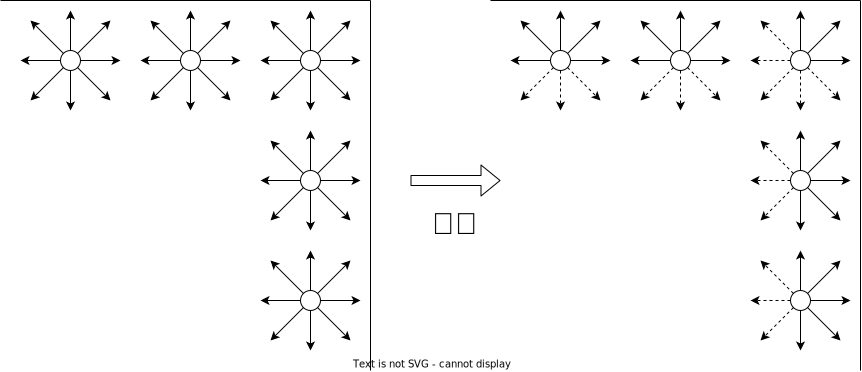
\includegraphics[width=13cm]{./how_to_assemble/figs/edge_streaming.drawio.svg.eps}
  \caption{外枠1マス分の仮想粒子の分布関数}
  \label{fig:edge-streaming}
\end{figure}

\subsection{時系列性のあるモデル}
実験で用いたモデルには入力データの時系列性を反映させるため,更にリカレントな重みを導入した.図\ref{fig:time-series-model}では本モデルの概要を示す.このモデルでは,$\Delta T$おきの時系列データが入力されたとき,それぞれの時刻に対して$\Delta T$後の時系列データを予測する.

\begin{figure}[tbp]
  \centering
  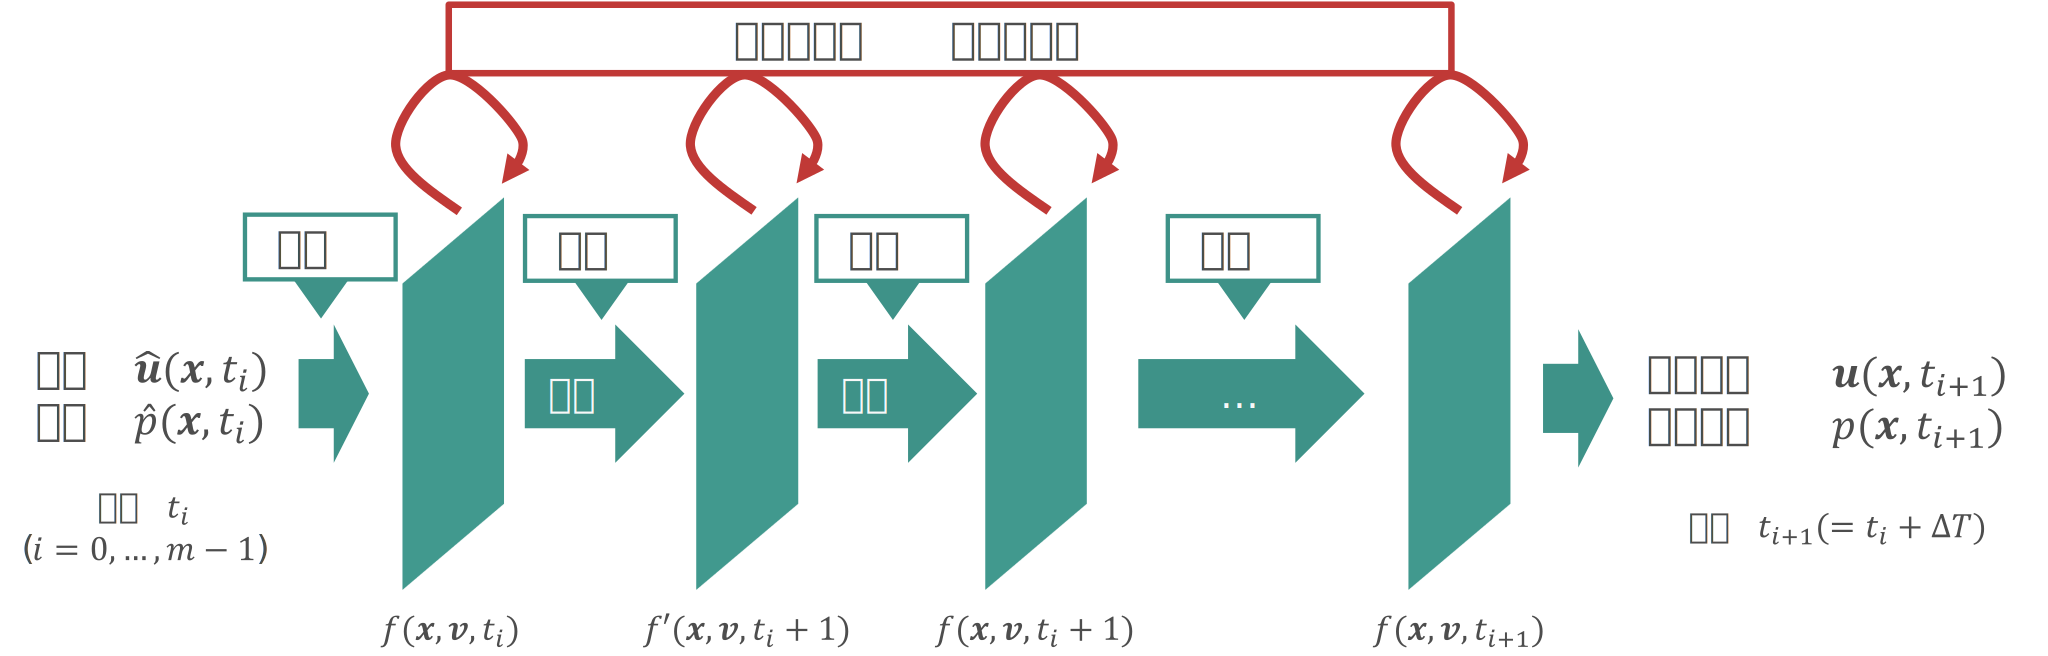
\includegraphics[width=13cm]{./how_to_assemble/figs/recurrent_model.svg.eps}
  \caption{時系列性のあるモデルの概要図}
  \label{fig:time-series-model}
\end{figure}

まずこの図に書かれるように,記号を再定義する.時系列データの長さを$n$とする.そして無次元時刻$t_0$から$t_n$までの$\Delta t$おきの実測時系列データを
\begin{equation}
    \left(\hat{\bm{u}}(\bm{x}, t_0), \hat{\rho}(\bm{x}, t_0)\right),
    \left(\hat{\bm{u}}(\bm{x}, t_1), \hat{\rho}(\bm{x}, t_1)\right),
    \cdots,
    \left(\hat{\bm{u}}(\bm{x}, t_n), \hat{\rho}(\bm{x}, t_n)\right)
  \label{eq:time-series-input}
\end{equation}
ただし,
\begin{equation}
  t_i = t_0 + i \Delta T \hspace{10pt} (0 \leq i \leq n)
\end{equation}
のように表す.なお,$\hat{\bm{u}}(\bm{x}, t_i)$は実測の無次元流速,$\hat{\rho}(\bm{x}, t_i)$は実測の無次元圧力を表す($0 \leq i \leq n$).更に,時刻$t_i$ $(0 \leq i \leq n-1)$のデータが入力されたときの内部における時刻$t_i + t$($0 \leq t \leq \Delta T$)の衝突(並進)後の仮想粒子の分布関数とそれから式(\ref{eq:lbm-macro-velocity}), (\ref{eq:lbm-macro-density})によって得られる巨視的な流速,圧力をそれぞれ
\begin{equation}
  f_i^{(\prime)}(\bm{x}, \bm{v}, t)
  \label{eq:time-series-f}
\end{equation}
\begin{equation}
  \bm{u}_i^{(\prime)}(\bm{x}, t)
  \label{eq:time-series-u}
\end{equation}
\begin{equation}
  \rho_i^{(\prime)}(\bm{x}, t)
  \label{eq:time-series-rho}
\end{equation}
と表すことにする.局所平衡分布関数$f_i^{eq}(\bm{x}, \bm{v}, t)$も同様である.

まずはこの時系列性があるモデルの入出力を概観する.このモデルのタスクは,$(\hat{\bm{u}}(\bm{x}, t_i), \hat{\rho}(\bm{u}, t_i))$が$i = 0$から$i = n-1$まで順次与えられたときにそれぞれに対して$(\hat{\bm{u}}(\bm{x}, t_{i+1}), \hat{\rho}(\bm{x}, t_{i+1}))$を予測することである.モデルの予測流速と圧力は,式(\ref{eq:time-series-u}), (\ref{eq:time-series-rho})から$\bm{u}_i(\bm{x}, \Delta T)$,$\rho_i(\bm{x}, \Delta T)$として得られ,式(\ref{eq:deep-learning-loss})より二乗損失は次のように表される.
\begin{equation}
  E = \sum_{\substack{\bm{x} \\ 0 \leq i \leq n-1}} 
  \left\| \bm{u}_i(\bm{x}, \Delta T) - \hat{\bm{u}}(\bm{x}, t_{i+1}) \right\|^2 +
  \left| \rho_i(\bm{x}, \Delta T) - \hat{\rho}(\bm{x}, t_{i+1}) \right|^2
  \label{eq:error-function-time-series}
\end{equation}

 さて,このモデルでは重みづけられた並進の式(\ref{eq:weighted-streaming})は更に重み成分$w'_{\rm{recur}}(\bm{x}, \bm{v}, t)$が加えられ次のように拡張される(ここで,各重みの変数$(\bm{x}, \bm{v}, t)$は省略してあることに注意せよ).
\begin{equation}
  f_i'(\bm{x}+\bm{v}, \bm{v}, t) =
  \begin{dcases}
    w'_{\rm{const}} + w'_{\rm{fprev}} f_i(\bm{x}, \bm{v}, t)
    & (i = 0) \\
    \begin{split}
      & w'_{\rm{recur}} f_{i-1}(\bm{x} + \bm{v}, \bm{v}, t) \\
      & \qquad + (1 - w'_{\rm{recur}})
      \left(
        w'_{\rm{const}} + w'_{\rm{fprev}} f_i(\bm{x}, \bm{v}, t)
      \right)
    \end{split}
    & (0 < i \leq n-1)
  \end{dcases}
  \label{eq:weighted-streaming-time-series}
\end{equation}

続いて,重みづけられた衝突の式(\ref{eq:weighted-collision}), (\ref{eq:weighted-equilibrium})には更に重み成分$w_{\rm{recur}}(\bm{x}, \bm{v}, t)$が加えられそれぞれ次のように拡張される(こちらも各重みの変数$(\bm{x}, \bm{v}, t)$を省略した).
\begin{equation}
  f_i(\bm{x}, \bm{v}, t + 1) = \\
  \begin{dcases}
    w_{\rm{fprev}} f_i'(\bm{x}, \bm{v}, t)
    + (1 - w_{\rm{fprev}}) f_i^{eq}(\bm{x}, \bm{v}, t)
    & (i = 0) \\
    \begin{split}
      & w_{\rm{recur}} f_{i-1}(\bm{x}, \bm{v}, t + 1) \\
      & \hspace{5pt} + (1 - w_{\rm{recur}})
      \left(
        w_{\rm{fprev}} f_i'(\bm{x}, \bm{v}, t)
        + (1 - w_{\rm{fprev}}) f_i^{eq}(\bm{x}, \bm{v}, t)
      \right)
    \end{split}
    & (0 < i \leq n-1)
  \end{dcases}
  \label{eq:weighted-collision-time-series}
\end{equation}

\begin{equation}
\begin{split}
  f_i^{eq}(\bm{x}, \bm{v}, t) =
  &c_i(\bm{v}) \rho_i'(\bm{x}, t) \\
  &[ 1 + w_{\rm{vu}}\bm{v} \cdot \bm{u}_i'(\bm{x}, t) \\
  &+ w_{\rm{vxu}}\bm{v} \times \bm{u}_i'(\bm{x}, t) \\
  &+ w_{\rm{vu2}}(\bm{v} \cdot \bm{u}_i'(\bm{x}, t))^2 \\
  &+ w_{\rm{u2}}\bm{u}_i'(\bm{x}, t)^2 ]
\end{split}
  \label{eq:weighted-equilibrium-time-series}
\end{equation}

以上のようにしてリカレントな重み成分をもつ時系列性のあるモデルを構築した.


\chapter{提案モデルによる日本近辺の風速予測\label{chap:experiments}}
本論文では,提案モデルの性能検証のために日本近辺の風速予測を実施した.また,性能の比較のためにCNNによるエンコーダ・デコーダとLSTMを用いたU-Net-likeなモデルを実装し,それぞれのモデルの性能を比較した.

\section{実験の概要 \label{section:exp-overview}}
ここに何をメトリクスとして取ったのかとかを書く

\section{利用したデータ及び学習条件 \label{section:exp-data-and-condition}}
\subsection{利用したデータ \label{subsection:exp-data}}
気象庁が提供している日本近辺の風速と気圧データを京都大学の生存圏データベース\cite{Seizonken2004}から入手した.このデータセットは図\ref{fig:exp-data-overview}に示す通り,日本近辺の北緯$22.4\tcdegree$から$47.6\tcdegree$まで,東経$120\tcdegree$から$150\tcdegree$までの領域をそれぞれ$0.05\tcdegree \times 0.0625\tcdegree$の細かさで等緯度等経度に区切り,各格子点上における風速と気圧を記録したものである\cite{JMBSC2022}.すなわち,ある一時刻のデータは緯度経度について$505 \times 480$の行列となっており,ある一点には風速の南北方向成分$(\mathrm{m/s})$, 風速の東西方向成分$(\mathrm{m/s})$, 気圧$(\mathrm{hPa})$の3つの値が記録されている.
\begin{figure}[bp]
  \centering
  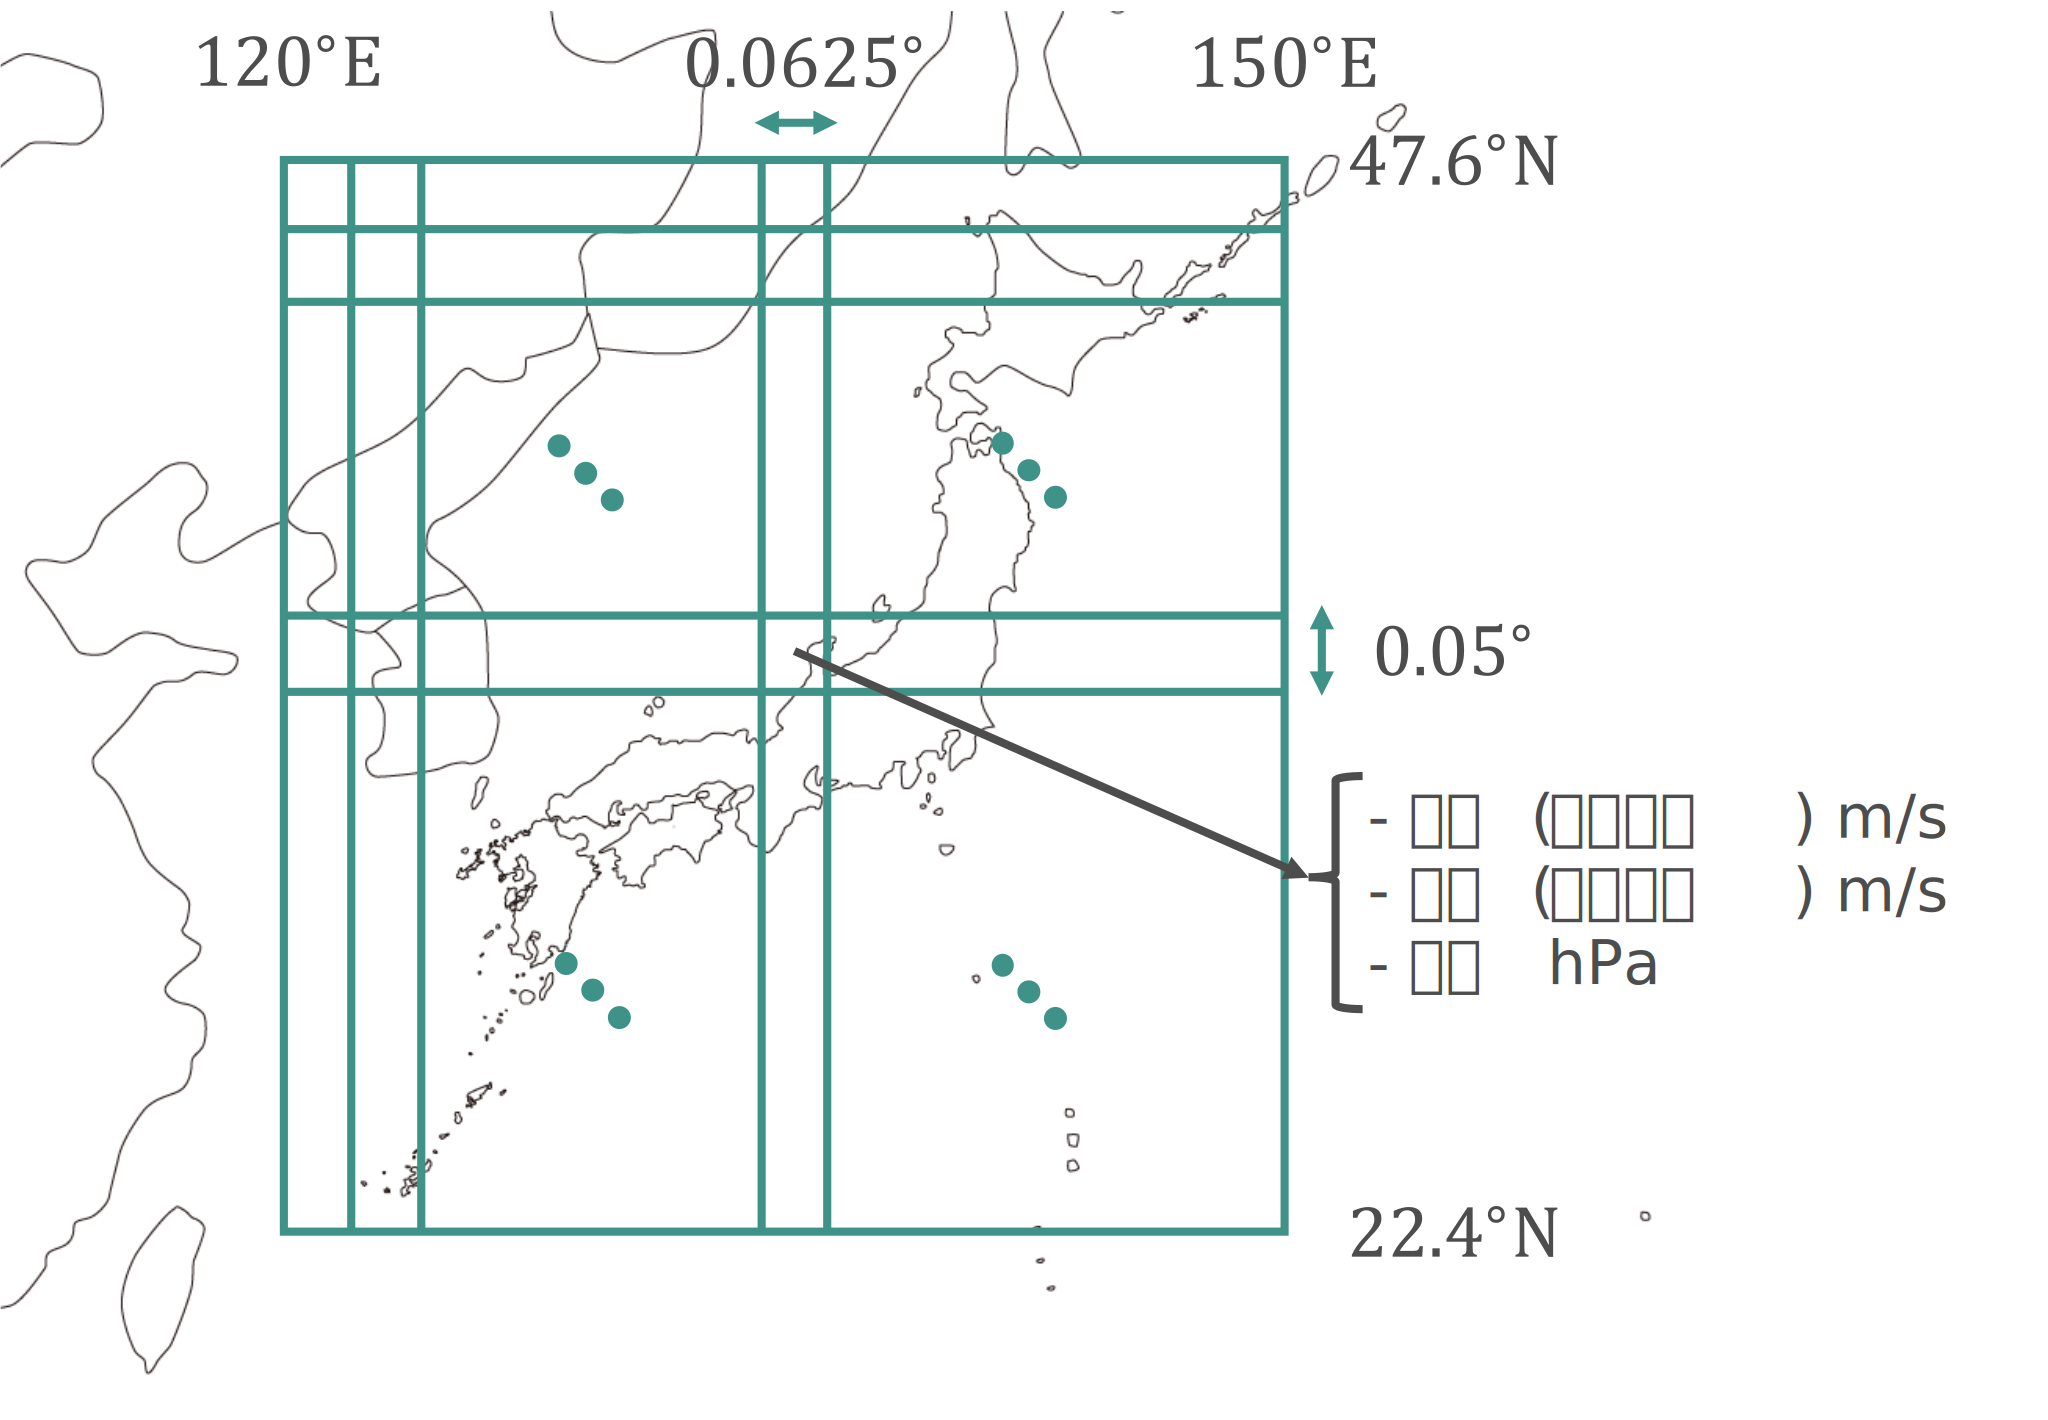
\includegraphics[width=0.6\linewidth]{./experiments/figs/data_overview.svg.eps}
  \caption{気象庁が提供している日本近辺の風速と気圧データの領域}
  \label{fig:exp-data-overview}
\end{figure}

今回の時系列データは3時間間隔であり,(前日の)21:00, 0:00, 3:00の3時刻分のデータを入力として6:00の時刻の風速を予測するというタスクを行った.すなわち,式(\ref{eq:time-series-input})において$n=5$,式(\ref{eq:time-series-t})において無次元時刻$\Delta T$は$3[\mathrm{h}]$相当である.この4時刻分の時系列データを2011年1月1日から2020年12月31日までの3650日分用意し(統計を取る際の簡便化のために閏日は除いてある),\ref{subsection:exp-data-preprocessing}で述べる処理をする前の全体のデータセットとした.

処理前の全体のデータセットの詳細な統計量を表\ref{todo:table:exp-pre-data-statistics}に示す.

\subsection{データの前処理 \label{subsection:exp-data-preprocessing}}
\ref{subsection:exp-data}項で述べたデータセットをそのまま入出力として用いるのではなく,いくつかの前処理を実施した.その処理の詳細を以下に示す.

まず図\ref{fig:exp-averaging}に示すように,$505 \times 480$の行列を更に$10 \times 10$の格子によって区切り,この格子内で風速と気圧を平均化することで$50 \times 48$のサイズまで落とした.なお,端数分は切り捨てている.これは,提案モデルの格子の大きさを適切に設定することで,3時間で変化する風速の空間的な変化を捉えることができると考えたためである.このデータセットを改めて全体のデータセットとした.このデータセットの詳細な統計量を表\ref{todo:table:exp-data-statistics}に示す.

\begin{figure}[bp]
  \centering
  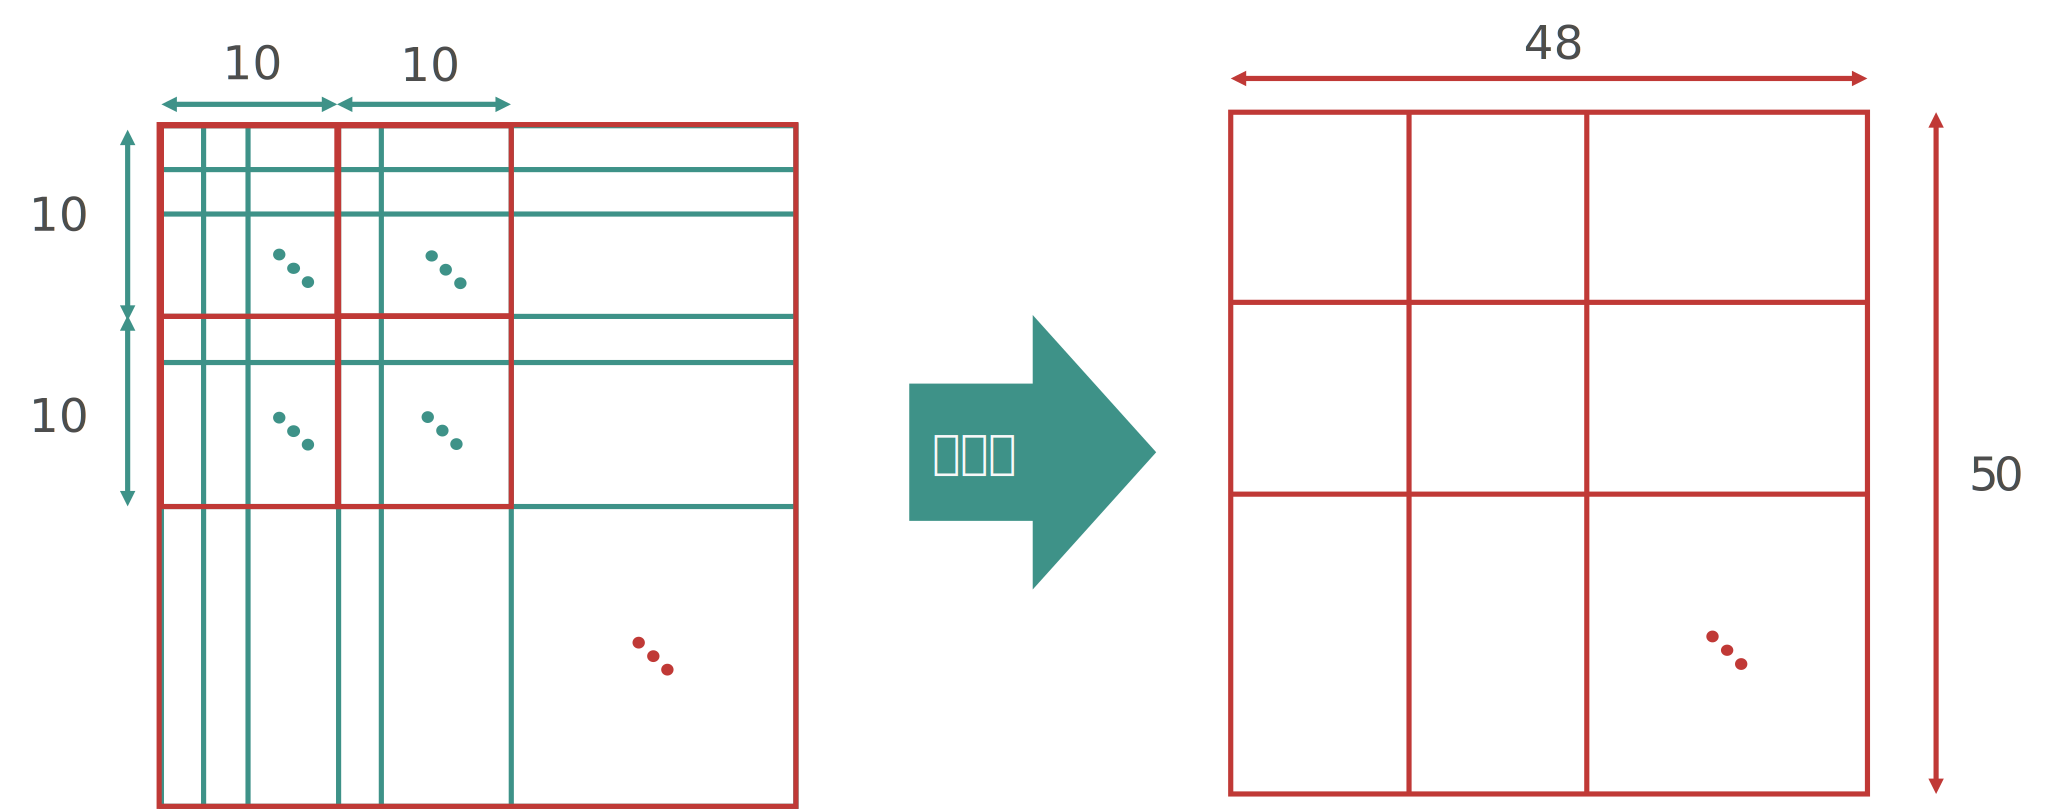
\includegraphics[width=0.8\linewidth]{./experiments/figs/average_pool.svg.eps}
  \caption{風速と気圧の平均化}
  \label{fig:exp-averaging}
\end{figure}

%todo 標準化についても時間があればここで触れる

\subsection{学習条件 \label{subsection:exp-condition}}

続いて,モデルの詳細な学習条件について述べる.まず,提案モデルの原理について\ref{subsection:time-series-model}項で述べたがここでは具体的な数値を示しながらモデルのアーキテクチャを見る.図\ref{fig:exp-model-architecture}に示したように,このモデルでは並進と衝突をそれぞれ5回行った(緑の実線矢印が並進を表し,緑の破線矢印が衝突を表している).すなわち式(\ref{eq:time-series-t})において$\Delta T = 5$である.\ref{subsection:time-series-less-model}項で述べた通り衝突の回数分だけ外枠が削られるため,図中の赤破線によって強調しているように出力層の大きさは入力層に比べて東西南北の端$5$マス分減少している.

\begin{figure}[bp]
  \centering
  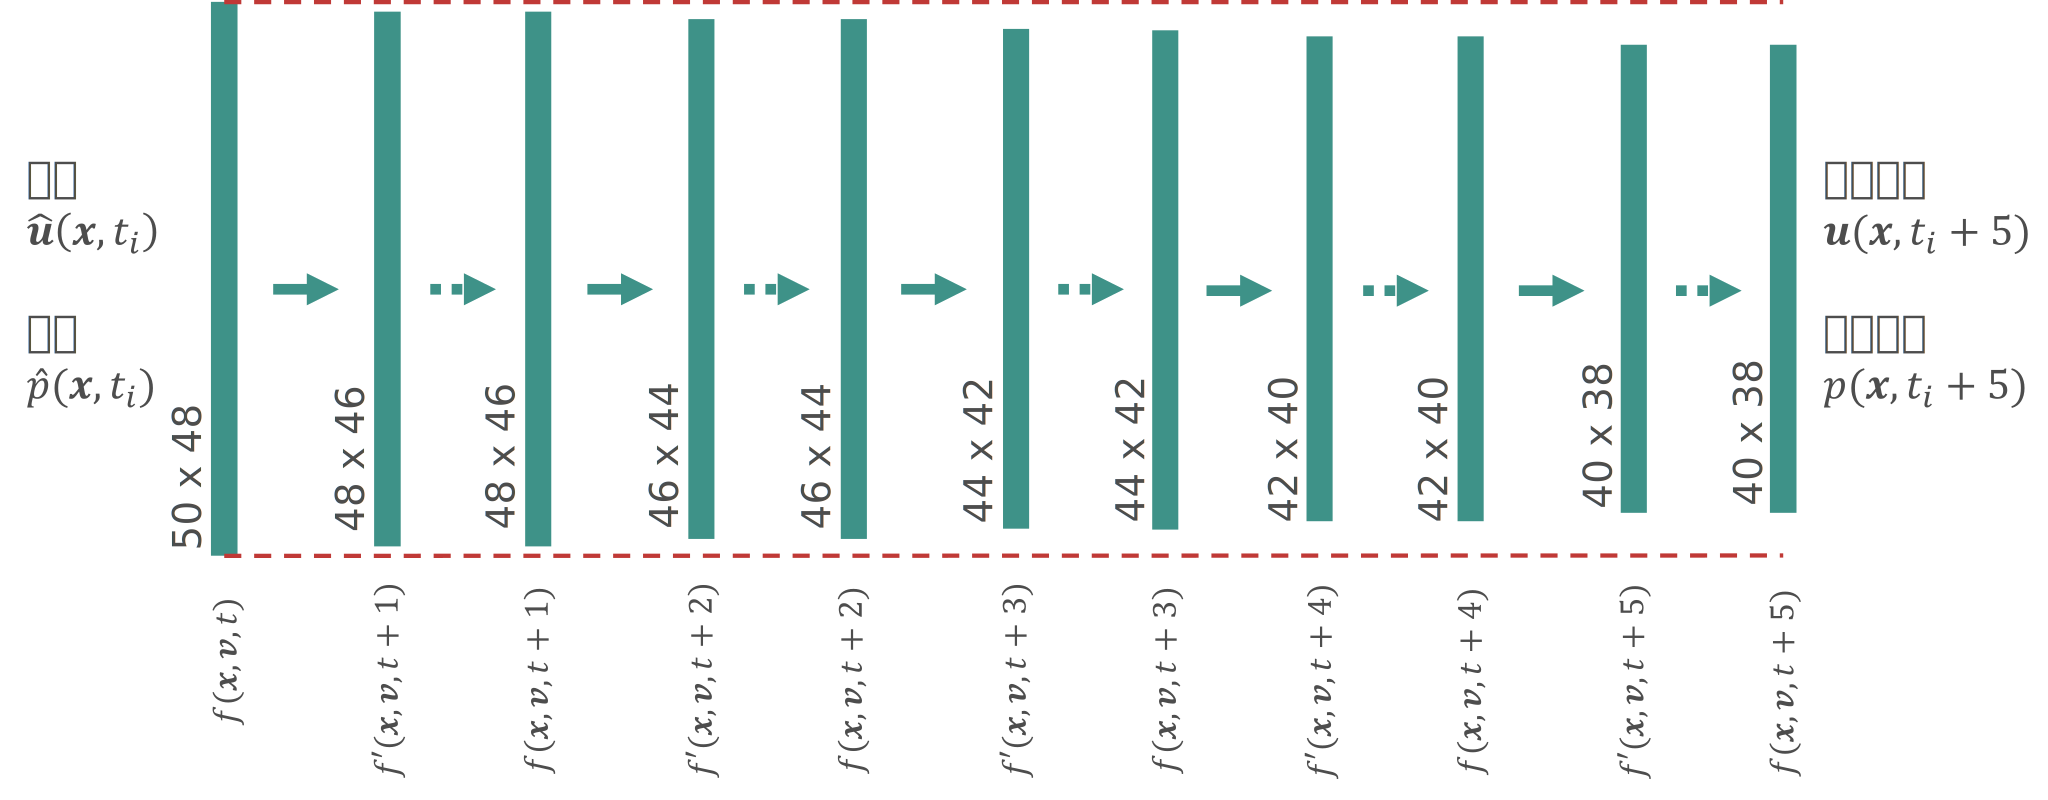
\includegraphics[width=0.85\linewidth]{./experiments/figs/model_architecture.svg.eps}
  \caption{モデルのアーキテクチャ}
  \label{fig:exp-model-architecture}
\end{figure}

% 損失関数について,式(\ref{eq:time-series-loss})に示したがここでは風速の精度を重視するため,式(\ref{eq:time-series-loss})の第1項の重みを$1$,第2項の重みを$0.1$とした.
%todo: なんで気圧の予測はしないのか聞かれたらこの辺も追記する

提案モデルの学習にはAdam\cite{Kingma2014AdamAM}を用いた.学習率は$10^{-3}$とし,ミニバッチサイズは$16$とした.全体のデータセットを2920日分と730日分に分けそれぞれを学習用データと検証用データとした.学習は$500$エポック行い,かかった時間は約8時間であった.実行環境にはGoogle Colaboratory\cite{GoogleColaboratory}を用い,GPUはTesla T4を用いた.また提案モデルの構築にはPyTorch\cite{NEURIPS2019-9015}を用い,自動微分による学習を行った.
% 損失の重み付けについて書く(速度に重みを強くつけた)

% 学習するLBM
% 学習しないLBM
% U-Net-Like
% で,
% 全体のRMSE, ME
% 座標ごとのRMSE, ME 東西方向, 南北方向,風速, 風向
% 時間ごとのRMSE, ME 上のそれぞれ
% 特徴的な日の座標のRMSE, ME 上のそれぞれ
% 
% それぞれのRMSE比についても書く(4.4のほうかな?)

\section{実験結果 \label{section:exp-results}}

\section{物理的な構造を含まない深層学習モデルによる実験結果 \label{section:exp-results-without-physicial-structure}}

\section{考察 \label{section:exp-discussion}}
% 平均化についてもふれて,どうやってアップスケーリングするか
% 短所として外枠の風速が予測できないことにふれる

\bibliographystyle{junsrt}
\bibliography{refs}

\end{document}